%!TEX root = ../dissertation.tex

\section*{Thesis overview}

%!TEX root = ../dissertation.tex

\section*{Thesis contents}

The \textbf{introduction} of the thesis contains the relevance of the research, a formulation of the aim, objectives, principal statements of the thesis, as well as scientific novelty, theoretical and practical significance of the work.

\textbf{\underline{Chapter 1}} presents an analytical review of the research domain and existing research results in the area of deterministic finite automata inference.
It also introduces the terminology, main definitions and known results from a number of topics in informatics that are necessary for the description of methods and algorithms proposed in the thesis.

\insectionen{\ref{sec:review:sat}} a formal setting of the Boolean satisfiability problem is given along with necessary definitions and
a brief description of the main approaches for solving this problem.
Also this section describes an approach to solving NP-hard problems through their polynomial-time reduction to the Boolean satisfiability problem.
Moreover, a brief overview of existing software tools for solving the Boolean satisfiability problem (SAT solvers) is given.

A Boolean formula is in \emph{conjunctive normal form} (CNF) if it is a conjunction of clauses, where each clause is a disjunction 
of literals.
The \emph{Boolean satisfiability problem} (\emph{satisfiability problem}, SAT) consists of determining, whether for a given Boolean formula in CNF there exists a satisfying assignment: a set of values of its variables for which the formula is true.
SAT is the historically first problem for which NP-completenss has been proved: any problem from NP can be reduced to SAT in polynomial time.
This fact explains the relevance of the development of more and more efficient SAT solvers.
The research community annually holds competitions to determine the best SAT solver; this fact also contributes to continuous development of this area.
The basis of all modern SAT solvers is the \emph{conflict driven clause learning}~(CDCL) strategy.

The approach to solving problems from NP, in which a reduction to SAT is devised and then a SAT solver is used to find a satisfying
assignment of the constructed Boolean formula, often turns out to be much more efficient and simpler than the development of a practically applicable method that directly solves the original problem.
Another important advantage of this approach is the fact that it is enough to write a reduction to the SAT once, and then, without applying any effort, use the progress of SAT solvers, choosing the most efficient one.



\insectionen{\ref{sec:review:dfa-inf}} basic concepts of deterministic finite automata and the formulation of the problem of inferring deterministic finite automata from behavior examples are given.
Behavior examples for some DFA $\mathcal{D}$ are defined as two sets of words $S_{+}$ and $S_{-}$ over the symbols of the DFA's alphabet, such that all words from $S_{+}$ belong the the language $\mathcal{L}\left(\mathcal{D}\right)$ and must be accepted by the DFA, and all words from $S_{-}$ do not belong to the language $\mathcal{L}\left(\mathcal{D}\right)$ 
and must be rejected by  the DFA.
The problem of DFA inference from behavior examples consists in finding a DFA of minimal size (with the minimal number of states) that
satisfies given behavior examples.
Previously it has been shown that this problem is NP-complete, as well as the problem of finding a DFA of any given size that satisfies given behavior examples.
An example of a DFA that satisfies behavior examples $S_{+} = \{aba, bb, bba\}$ and $S_{-} = \{b, ba\}$ is shown in Figure~\ref{syn-en:img:dfa-ex}.
One can notice that an automaton with two states satisfying sets $S_{+}$ and $S_{-}$ does not exist.
\begin{figure}[ht]
  \centering
  \ifafour
    \begin{tikzpicture}[
    ->, % makes the edges directed
    >=stealth', % makes the arrow heads bold
    node distance=2.5cm, % specifies the minimum distance between two nodes. Change if necessary.
    every state/.style={thick, fill=gray!10, minimum size = 0pt}, % sets the properties for each ’state’ node
    initial text=$ $, % sets the text that appears on the start arrow
    double distance between line centers=2pt
]
    \node[state, initial, accepting] (q1) {$1$};
    \node[state, accepting] (q2) [above of=q1, xshift=2.5cm/2, yshift=-0.4cm] {$2$};
    \node[state] (q3) [right of=q1] {$3$};

    \path
        (q1) edge [bend right=10, below] node [xshift=2pt] {a} (q2)
        (q2) edge [bend right=10, above] node [xshift=-2pt] {b} (q1)
        (q1) edge [bend right=10, below] node {b} (q3)
        (q3) edge [bend right=10, above] node [xshift=2pt] {b} (q1)
        (q2) edge [above] node [xshift=2pt] {a} (q3)
        (q3) edge [loop above] node {a} (q3)
        ;
\end{tikzpicture}
    % 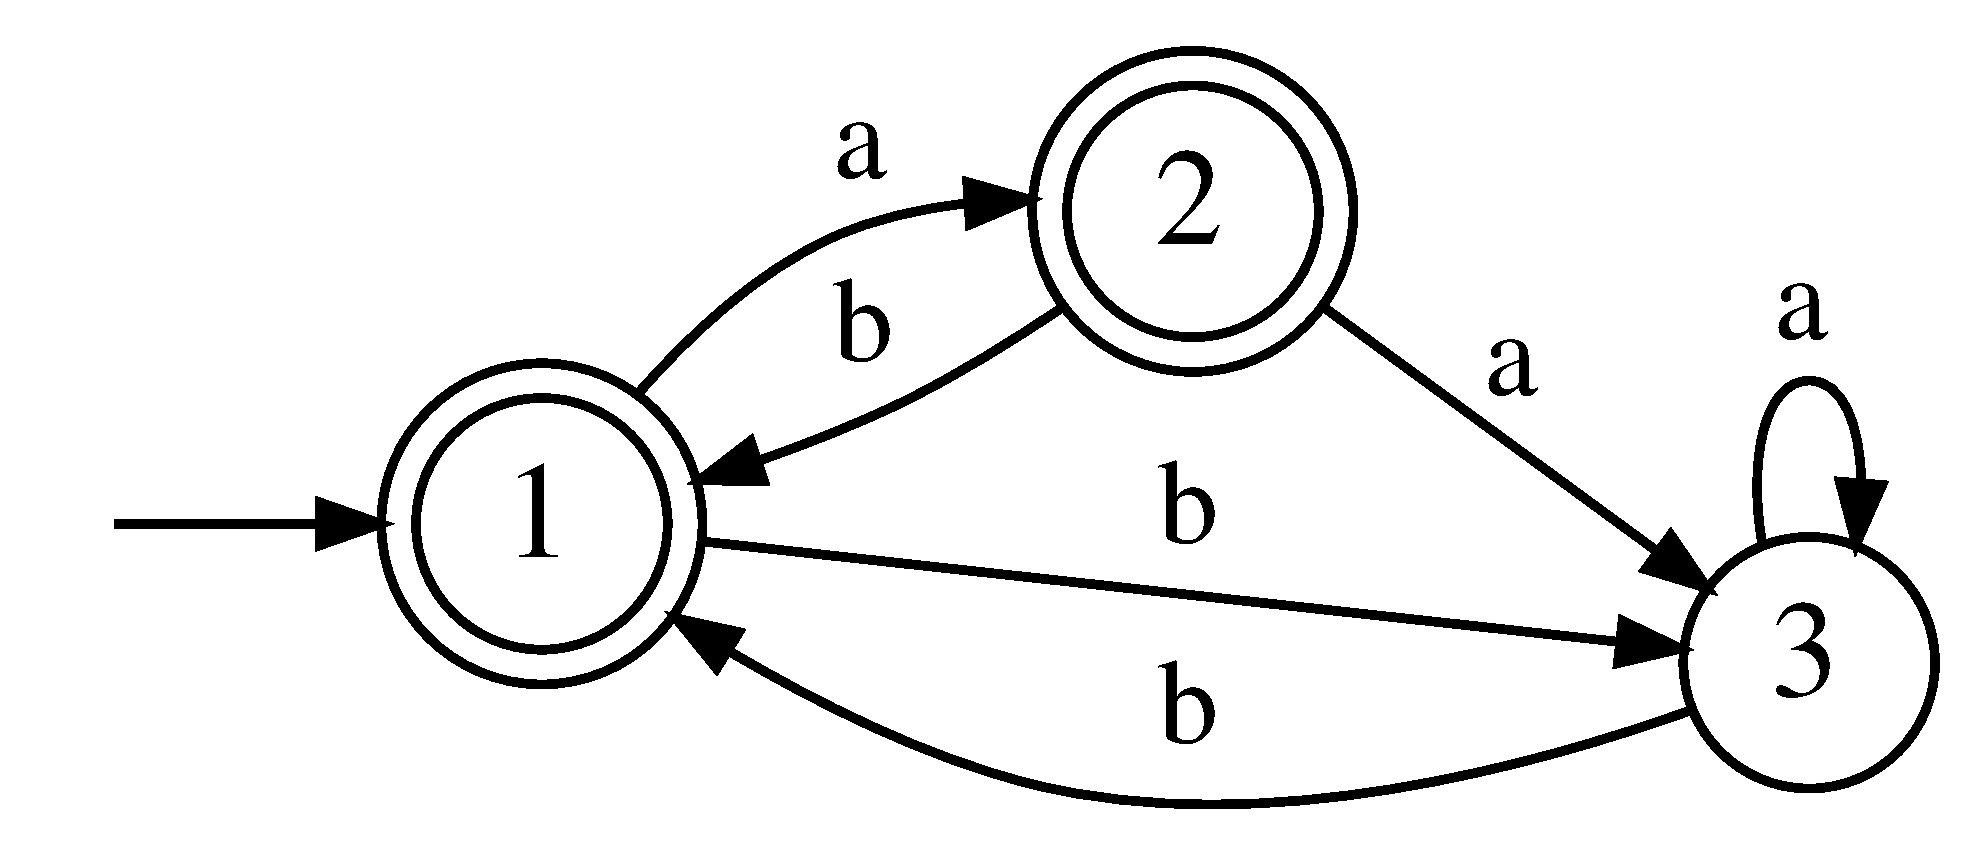
\includegraphics[scale=0.16]{img/datamod/FIG1.eps}
  \else
    \begin{tikzpicture}[
    ->, % makes the edges directed
    >=stealth', % makes the arrow heads bold
    node distance=1.9cm, % specifies the minimum distance between two nodes. Change if necessary.
    every state/.style={thick, fill=gray!10, minimum size = 0pt}, % sets the properties for each ’state’ node
    initial text=$ $, % sets the text that appears on the start arrow
]
    \node[state, initial, accepting] (q1) {$1$};
    \node[state, accepting] (q2) [above of=q1, xshift=1.9cm/2, yshift=-0.3cm] {$2$};
    \node[state] (q3) [right of=q1] {$3$};

    \path
        (q1) edge [bend right=10, below] node [xshift=2pt] {a} (q2)
        (q2) edge [bend right=10, above] node [xshift=-2pt] {b} (q1)
        (q1) edge [bend right=10, below] node {b} (q3)
        (q3) edge [bend right=10, above] node {b} (q1)
        (q2) edge [above] node [xshift=2pt] {a} (q3)
        (q3) edge [loop above] node {a} (q3)
        ;
\end{tikzpicture}
  \fi
  \caption{An example of a minimal DFA satisfying behavior examples $S_{+} = \{aba, bb, bba\}$ and $S_{-} = \{b, ba\}$}
  \label{syn-en:img:dfa-ex}
\end{figure}

\textbf{Section~\ref{sec:review:heuristic-dfa-inf}} presents an overview of existing heuristic and metaheurstic methods and algorithms
for DFA inference from behavior examples.
Heuristic algorithms include the \emph{evidence-driven state merging}~(EDSM) algorithm.
Metaheuristic algorithms include evolutionary strategies, genetic algorithms, and ant colony optimization algorithms.

Note that the mentioned approaches are inexact: they do not guarantee that the found DFA contains the minimal number of states, and, in some cases, they do not even guarantee that any DFA satisfying the behavior examples will be found.

\insectionen{\ref{sec:review:sat-dfa-inf}} an overview of existing methods for inferring DFA from behavior examples based on reduction to SAT is given. Unlike heuristic and metaheuristic approaches, these methods are exact: it is guaranteed that the automaton corresponding to the behavior examples will be found in finite time and will contain the minimum possible number of states.

The first step of considered methods is the construction of the \emph{augmented prefix tree acceptor}~(APTA): a tree-like data structure 
based on the ordinary prefix tree, in which each vertex is either not marked, or marked as accepting or rejecting.
An example of an augmented prefix tree is shown in~\ref{syn-en:img:apta-ex}.

\begin{figure}[ht]
  \centering
  \ifafour
    \begin{tikzpicture}[
    ->, % makes the edges directed
    >=stealth', % makes the arrow heads bold
    node distance=2cm, % specifies the minimum distance between two nodes. Change if necessary.
    every state/.style={thick, fill=gray!10, minimum size = 0pt}, % sets the properties for each ’state’ node
    initial text=$ $, % sets the text that appears on the start arrow
    double distance between line centers=2pt
]
    \def\yshift{0.47cm}
    \def\xshift{0.26cm}

    \node[state, initial] (q1) {$1$};
    \node[state, fill=white, dashed, inner sep=9.7pt] (q5) [above right of=q1, yshift=-\yshift, xshift=\xshift] {};
    \node[state, inner sep=4.2pt] (dummy5) [above right of=q1, yshift=-\yshift, xshift=\xshift] {$5$};
    \node[state, accepting] (q6) [right of=q5] {$6$};
    \node[state, accepting] (q7) [right of=q6] {$7$};
    \node[state] (q2) [below right of=q1, yshift=\yshift, xshift=\xshift] {$2$};
    \node[state] (q3) [right of=q2] {$3$};
    \node[state, accepting] (q4) [right of=q3] {$4$};
    \node[state, fill=white, dashed, inner sep=9.7pt] (q8) [above of=q6, yshift=-0.78cm] {};
    \node[state, inner sep=4.2pt] (dummy8) [above of=q6, yshift=-0.78cm] {$8$};

    \path 
        (q1) edge [above] node {b} (q5)
        (q5) edge [below] node {b} (q6)
        (q6) edge [below] node {a} (q7)
        (q5) edge [above] node {a} (q8)
        (q1) edge [below] node {a} (q2)
        (q2) edge [below] node {b} (q3)
        (q3) edge [below] node {a} (q4)
        ;
\end{tikzpicture}
    %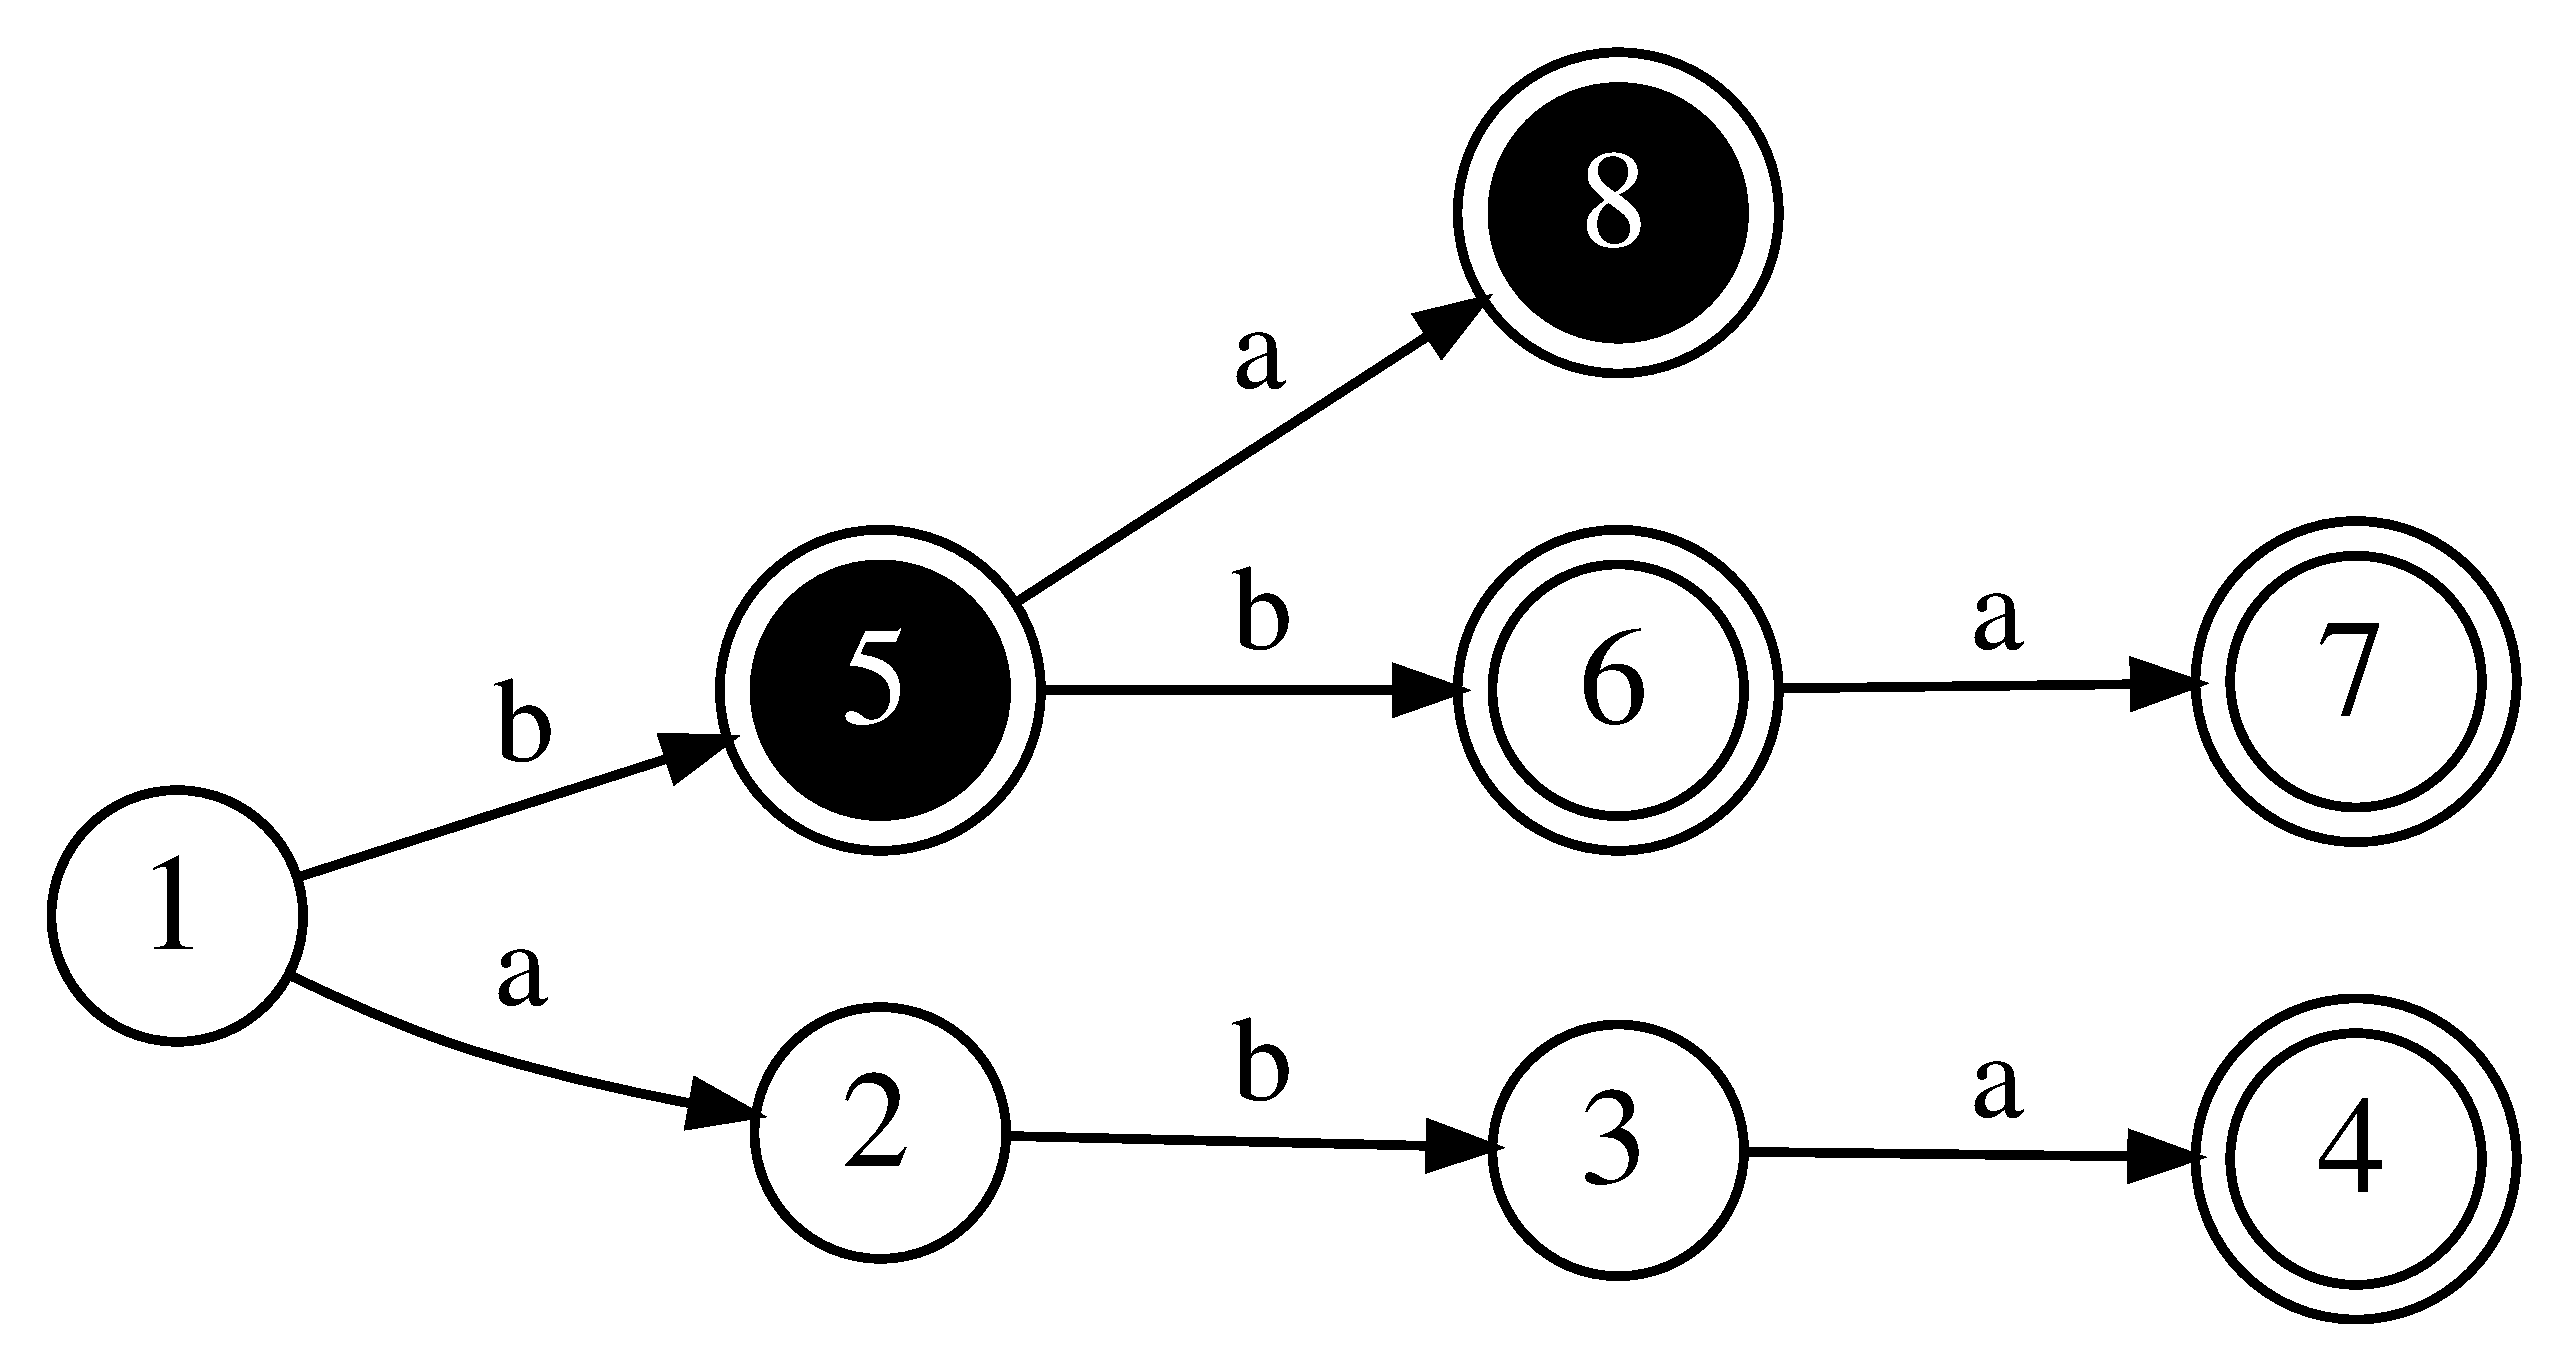
\includegraphics[scale=0.14]{img/datamod/FIG2a.eps}
  \else
    \begin{tikzpicture}[
    ->, % makes the edges directed
    >=stealth', % makes the arrow heads bold
    node distance=1.5cm, % specifies the minimum distance between two nodes. Change if necessary.
    every state/.style={thick, fill=gray!10, minimum size = 0pt}, % sets the properties for each ’state’ node
    initial text=$ $, % sets the text that appears on the start arrow
]
    \def\yshift{0.36cm}
    \def\xshift{0.2cm}

    \node[state, initial] (q1) {$1$};
    \node[state, dashed, inner sep=7pt] (q5) [above right of=q1, yshift=-\yshift, xshift=\xshift] {};
    \node[state, inner sep=3pt] (dummy5) [above right of=q1, yshift=-\yshift, xshift=\xshift] {$5$};
    \node[state, accepting] (q6) [right of=q5] {$6$};
    \node[state, accepting] (q7) [right of=q6] {$7$};
    \node[state] (q2) [below right of=q1, yshift=\yshift, xshift=\xshift] {$2$};
    \node[state] (q3) [right of=q2] {$3$};
    \node[state, accepting] (q4) [right of=q3] {$4$};
    \node[state, dashed, inner sep=7pt] (q8) [above of=q6, yshift=-0.58cm] {};
    \node[state, inner sep=3pt] (dummy8) [above of=q6, yshift=-0.58cm] {$8$};

    \path 
        (q1) edge [above] node {b} (q5)
        (q5) edge [below] node {b} (q6)
        (q6) edge [below] node {a} (q7)
        (q5) edge [above] node {a} (q8)
        (q1) edge [below] node {a} (q2)
        (q2) edge [below] node {b} (q3)
        (q3) edge [below] node {a} (q4)
        ;
\end{tikzpicture}
  \fi
  \caption{An example of a prefix tree acceptor constructed from behavior examples $S_{+} = \{aba, bb, bba\}$ and $S_{-} = \{b, ba\}$}
  \label{syn-en:img:apta-ex}
\end{figure}

Further, starting from a certain lower bound on the size (in the simplest case, from one) the search for an automaton of the current size corresponding to the constructed APTA is performed.
This process continues until a DFA is found that satisfies the given requirement.
Iterative increase of the automaton size guarantees that the found automaton has the minimum size.
As already mentioned, the problem of finding a DFA of a specific size for given behavior belongs to the NP class, and therefore can be solved by reducing it to some NP-hard problem.
Until recently, the most efficient method was considered to be \texttt{DFASAT}~\cite{heule-icgi10}, in which the authors
proposed to first reduce the DFA inference problem to graph coloring (color the APTA in the minimal number of colors in such a way that vertices of one color would be merged into one state), and then reduce graph coloring to SAT.
The scheme of the \texttt{DFASAT} method is shown in Figure~\ref{syn-en:img:dfasat-algo}.

\begin{figure}[ht]
  \centering
  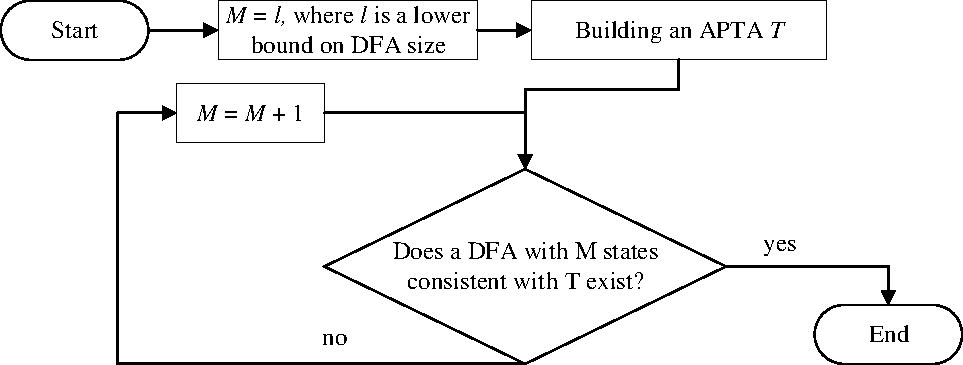
\includegraphics[scale=0.9]{img/ntv/basic-en.pdf}
  \caption{Scheme of \texttt{DFASAT}, an exact SAT-based method for DFA inference from given behavior examples}
  \label{syn-en:img:dfasat-algo}
\end{figure}

Authors of \texttt{DFASAT} use several approaches for search space reduction:
\begin{enumerate}
  \item adding several types of auxiliary clauses that do not influence the solution, but introduce additional constraints on possible variable values;
  \item construction of the consistency graph allowing finding in advance some pairs of vertices of the prefix tree that cannot be combined into one state of the automaton;
  \item construction of some large clique in the consistency graph and fixing the enumeration of this clique's vertices.
\end{enumerate}

Application of the aforementioned approaches yields a considerable increase of the efficiency of the original method, but they do not solve the fundamental problem of the existence
of isomorphic automata.
Two automata are called isomorphic if they differ only in the enumeration of states.
Thus, if a DFA contains $N$ states, then there exist $\mathcal{O}\left(N!\right)$ automata isomorphic to it.
Despite that isomorphic automata do not differ from a practical point of view, for a SAT solver they are distinct.

The solution for this problem was found by means of development of symmetry breaking predicates based on \emph{breadth-first search}~(BFS)~\cite{zakirzyanov2015LATA}.
Inclusion of such predicates in the Boolean formula fixes the enumeration of considered automata in the BFS order, allowing to consider only on representative of each isomorphism 
equivalence class.
The SAT encoding of these predicates requires $\mathcal{O}\left(M^{3} + M^{2} \times L^{2}\right)$ clauses, where $N$ is the size of the prefix tree and $M$ is the size of the sought DFA.
The proposed symmetry breaking predicates were used to develop a SAT-based DFA inference method that has been implemented in a software tool \texttt{DFA-Inductor}~\cite{dfa-inductor-en}. This SAT-based DFA inference method that uses BFS symmetry breaking predicates is the most efficient exact DFA inference method, and it is the basis of all methods developed 
in this thesis.
An example of a BFS-enumerated DFA is shown in Figure~\ref{syn-en:img:bfs:bfs-ex}, and Figure~\ref{syn-en:img:bfs:bfs-tree} shows the corresponding BFS traversal tree.

\begin{figure}[ht]
  \centering
  \subfloat[An example of a BFS-enumerated automaton\label{syn-en:img:bfs:bfs-ex}]{
    \ifafour
      \begin{tikzpicture}[
    ->, % makes the edges directed
    >=stealth', % makes the arrow heads bold
    node distance=2.76cm, % specifies the minimum distance between two nodes. Change if necessary.
    every state/.style={thick, fill=gray!10, minimum size = 0pt}, % sets the properties for each ’state’ node
    initial text=$ $, % sets the text that appears on the start arrow
    double distance between line centers=2pt
]
    \node[state, initial above, accepting] (q1) {$1$};
    \node[state] (q2) [below left of=q1, xshift=0.8cm] {$2$};
    \node[state] (q3) [below right of=q1] {$3$};
    \node[state, accepting] (q5) [below left of=q2] {$5$};
    \node[state] (q6) [below of=q2] {$6$};
    \node[state, accepting] (q4) [below right of=q2] {$4$};
    \node[state] (q7) [below right of=q3] {$7$};

    \path 
        (q1) edge [left] node {a} (q2)
        (q1) edge [loop right] node {b} (q1)
        (q1) edge [bend right=10, left] node {c} (q3)
        (q3) edge [bend right=10, right] node {c} (q1)
        (q5) edge [bend left=30, left] node {a,c} (q1)
        (q2) edge [above] node {b} (q5)
        (q2) edge [bend right=10, left] node {c} (q6)
        (q6) edge [bend right=10, right] node [xshift=-1pt] {b,c} (q2)
        (q2) edge [above] node {a} (q4)
        (q3) edge [left] node {a} (q4)
        (q3) edge [bend right=10, left] node {b} (q7)
        (q7) edge [bend right=10, right] node {a,b,c} (q3)
        (q5) edge [above] node {b} (q6)
        (q6) edge [loop below] node {a} (q6)
        (q4) edge [loop below] node {a,b,c} (q4)
        ;
\end{tikzpicture}
      % 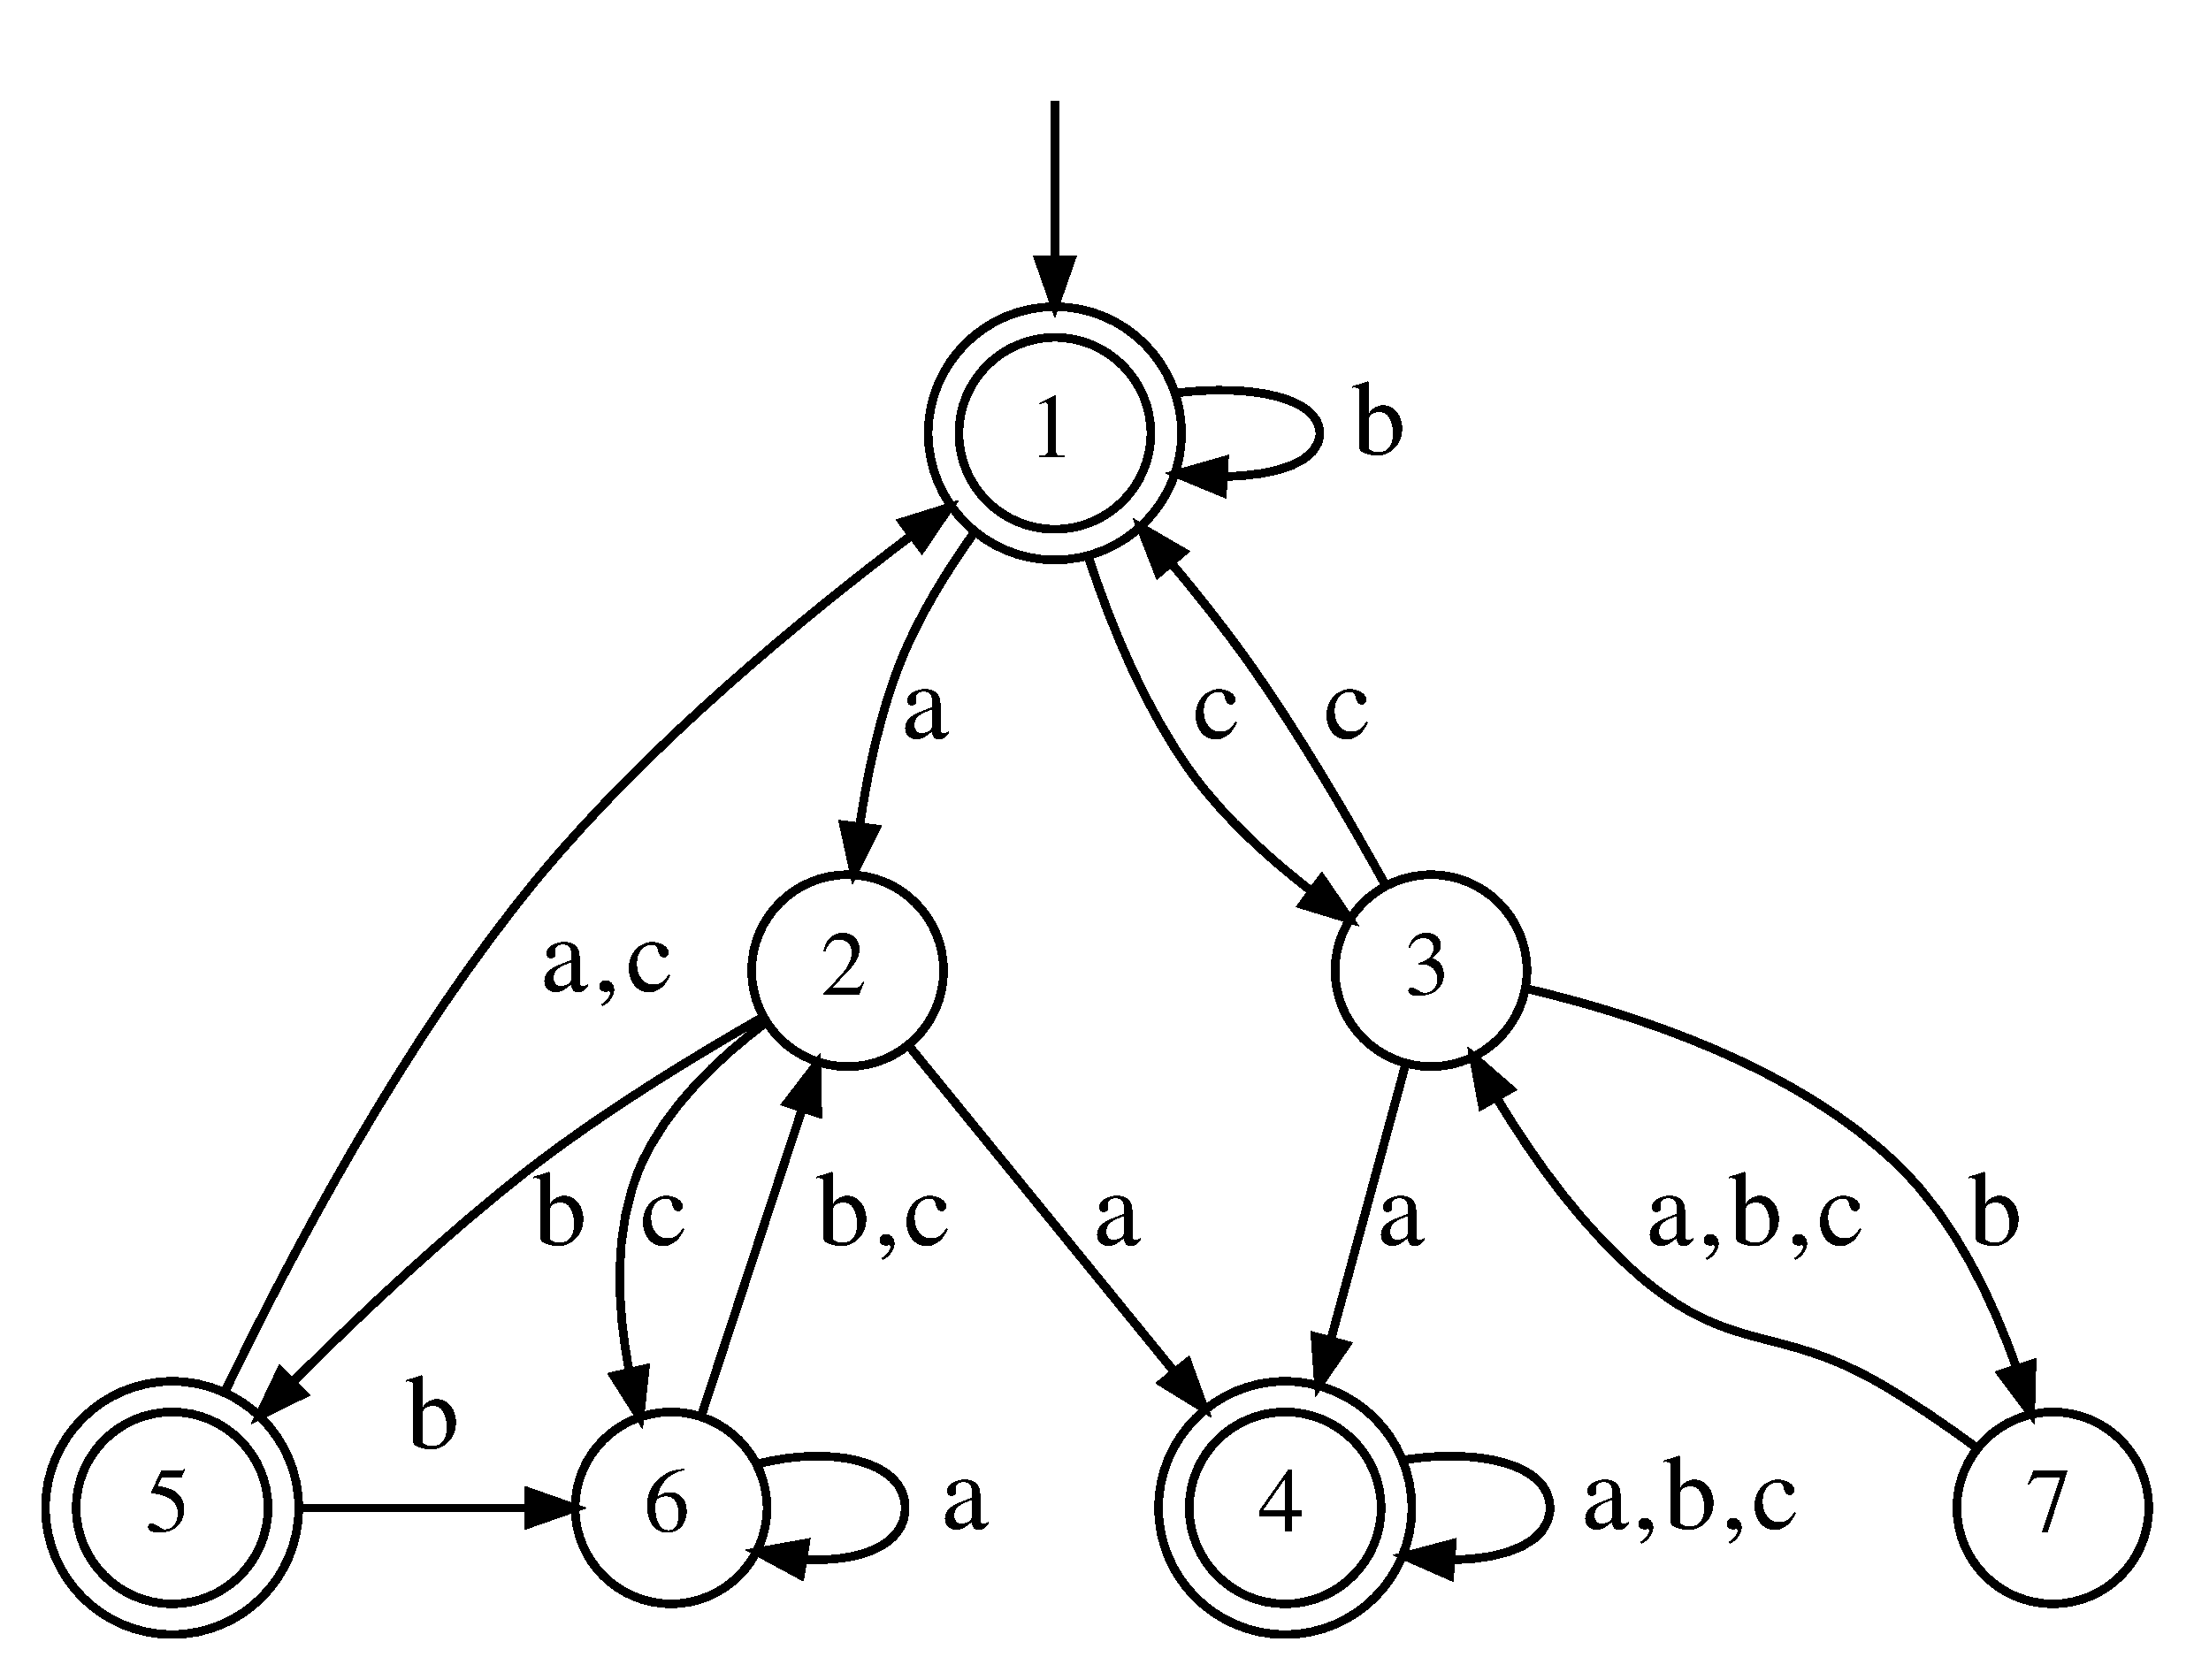
\includegraphics[scale=0.15]{img/datamod/BFS-example.eps}
    \else
      \begin{tikzpicture}[
    ->, % makes the edges directed
    >=stealth', % makes the arrow heads bold
    node distance=2.1cm, % specifies the minimum distance between two nodes. Change if necessary.
    every state/.style={thick, fill=gray!10, minimum size = 0pt}, % sets the properties for each ’state’ node
    initial text=$ $, % sets the text that appears on the start arrow
]
    \node[state, initial above, accepting] (q1) {$1$};
    \node[state] (q2) [below left of=q1, xshift=0.8cm] {$2$};
    \node[state] (q3) [below right of=q1] {$3$};
    \node[state, accepting] (q5) [below left of=q2] {$5$};
    \node[state] (q6) [below of=q2] {$6$};
    \node[state, accepting] (q4) [below right of=q2] {$4$};
    \node[state] (q7) [below right of=q3] {$7$};

    \path 
        (q1) edge [left] node {a} (q2)
        (q1) edge [loop right] node {b} (q1)
        (q1) edge [bend right=10, left] node {c} (q3)
        (q3) edge [bend right=10, right] node {c} (q1)
        (q5) edge [bend left=30, left] node {a,c} (q1)
        (q2) edge [above] node {b} (q5)
        (q2) edge [bend right=10, left] node {c} (q6)
        (q6) edge [bend right=10, right] node [xshift=-1pt] {b,c} (q2)
        (q2) edge [above] node {a} (q4)
        (q3) edge [left] node {a} (q4)
        (q3) edge [bend right=10, left] node {b} (q7)
        (q7) edge [bend right=10, right] node {a,b,c} (q3)
        (q5) edge [above] node {b} (q6)
        (q6) edge [loop below] node {a} (q6)
        (q4) edge [loop below] node {a,b,c} (q4)
        ;
\end{tikzpicture}
    \fi
  }
  \hfill
  \subfloat[BFS traversal tree for the automaton shown in Figure~\ref{syn-en:img:bfs:bfs-ex}\label{syn-en:img:bfs:bfs-tree}]{
    \ifafour
      \begin{tikzpicture}[
    ->, % makes the edges directed
    >=stealth', % makes the arrow heads bold
    node distance=2.23cm, % specifies the minimum distance between two nodes. Change if necessary.
    every state/.style={thick, fill=gray!10, minimum size = 0pt}, % sets the properties for each ’state’ node
    initial text=$ $, % sets the text that appears on the start arrow
    double distance between line centers=2pt
]
    \def\xshift{0.53cm}

    \node[state, initial above, accepting] (q1) {$1$};
    \node[state] (q2) [below left of=q1] {$2$};
    \node[state] (q3) [below right of=q1] {$3$};
    \node[state, accepting] (q5) [below of=q2]  {$5$};
    \node[state, accepting] (q4) [left of=q5, xshift=\xshift]  {$4$};
    \node[state] (q6) [right of=q5, xshift=-\xshift]  {$6$};
    \node[state] (q7) [below of=q3]  {$7$};

    \path
        (q1) edge [left] node {a} (q2)
        (q1) edge [right] node {c} (q3)
        (q2) edge [left] node {a} (q4)
        (q2) edge [left] node {b} (q5)
        (q2) edge [right] node {c} (q6)
        (q3) edge [right] node {b} (q7)
        ;
\end{tikzpicture}
    % 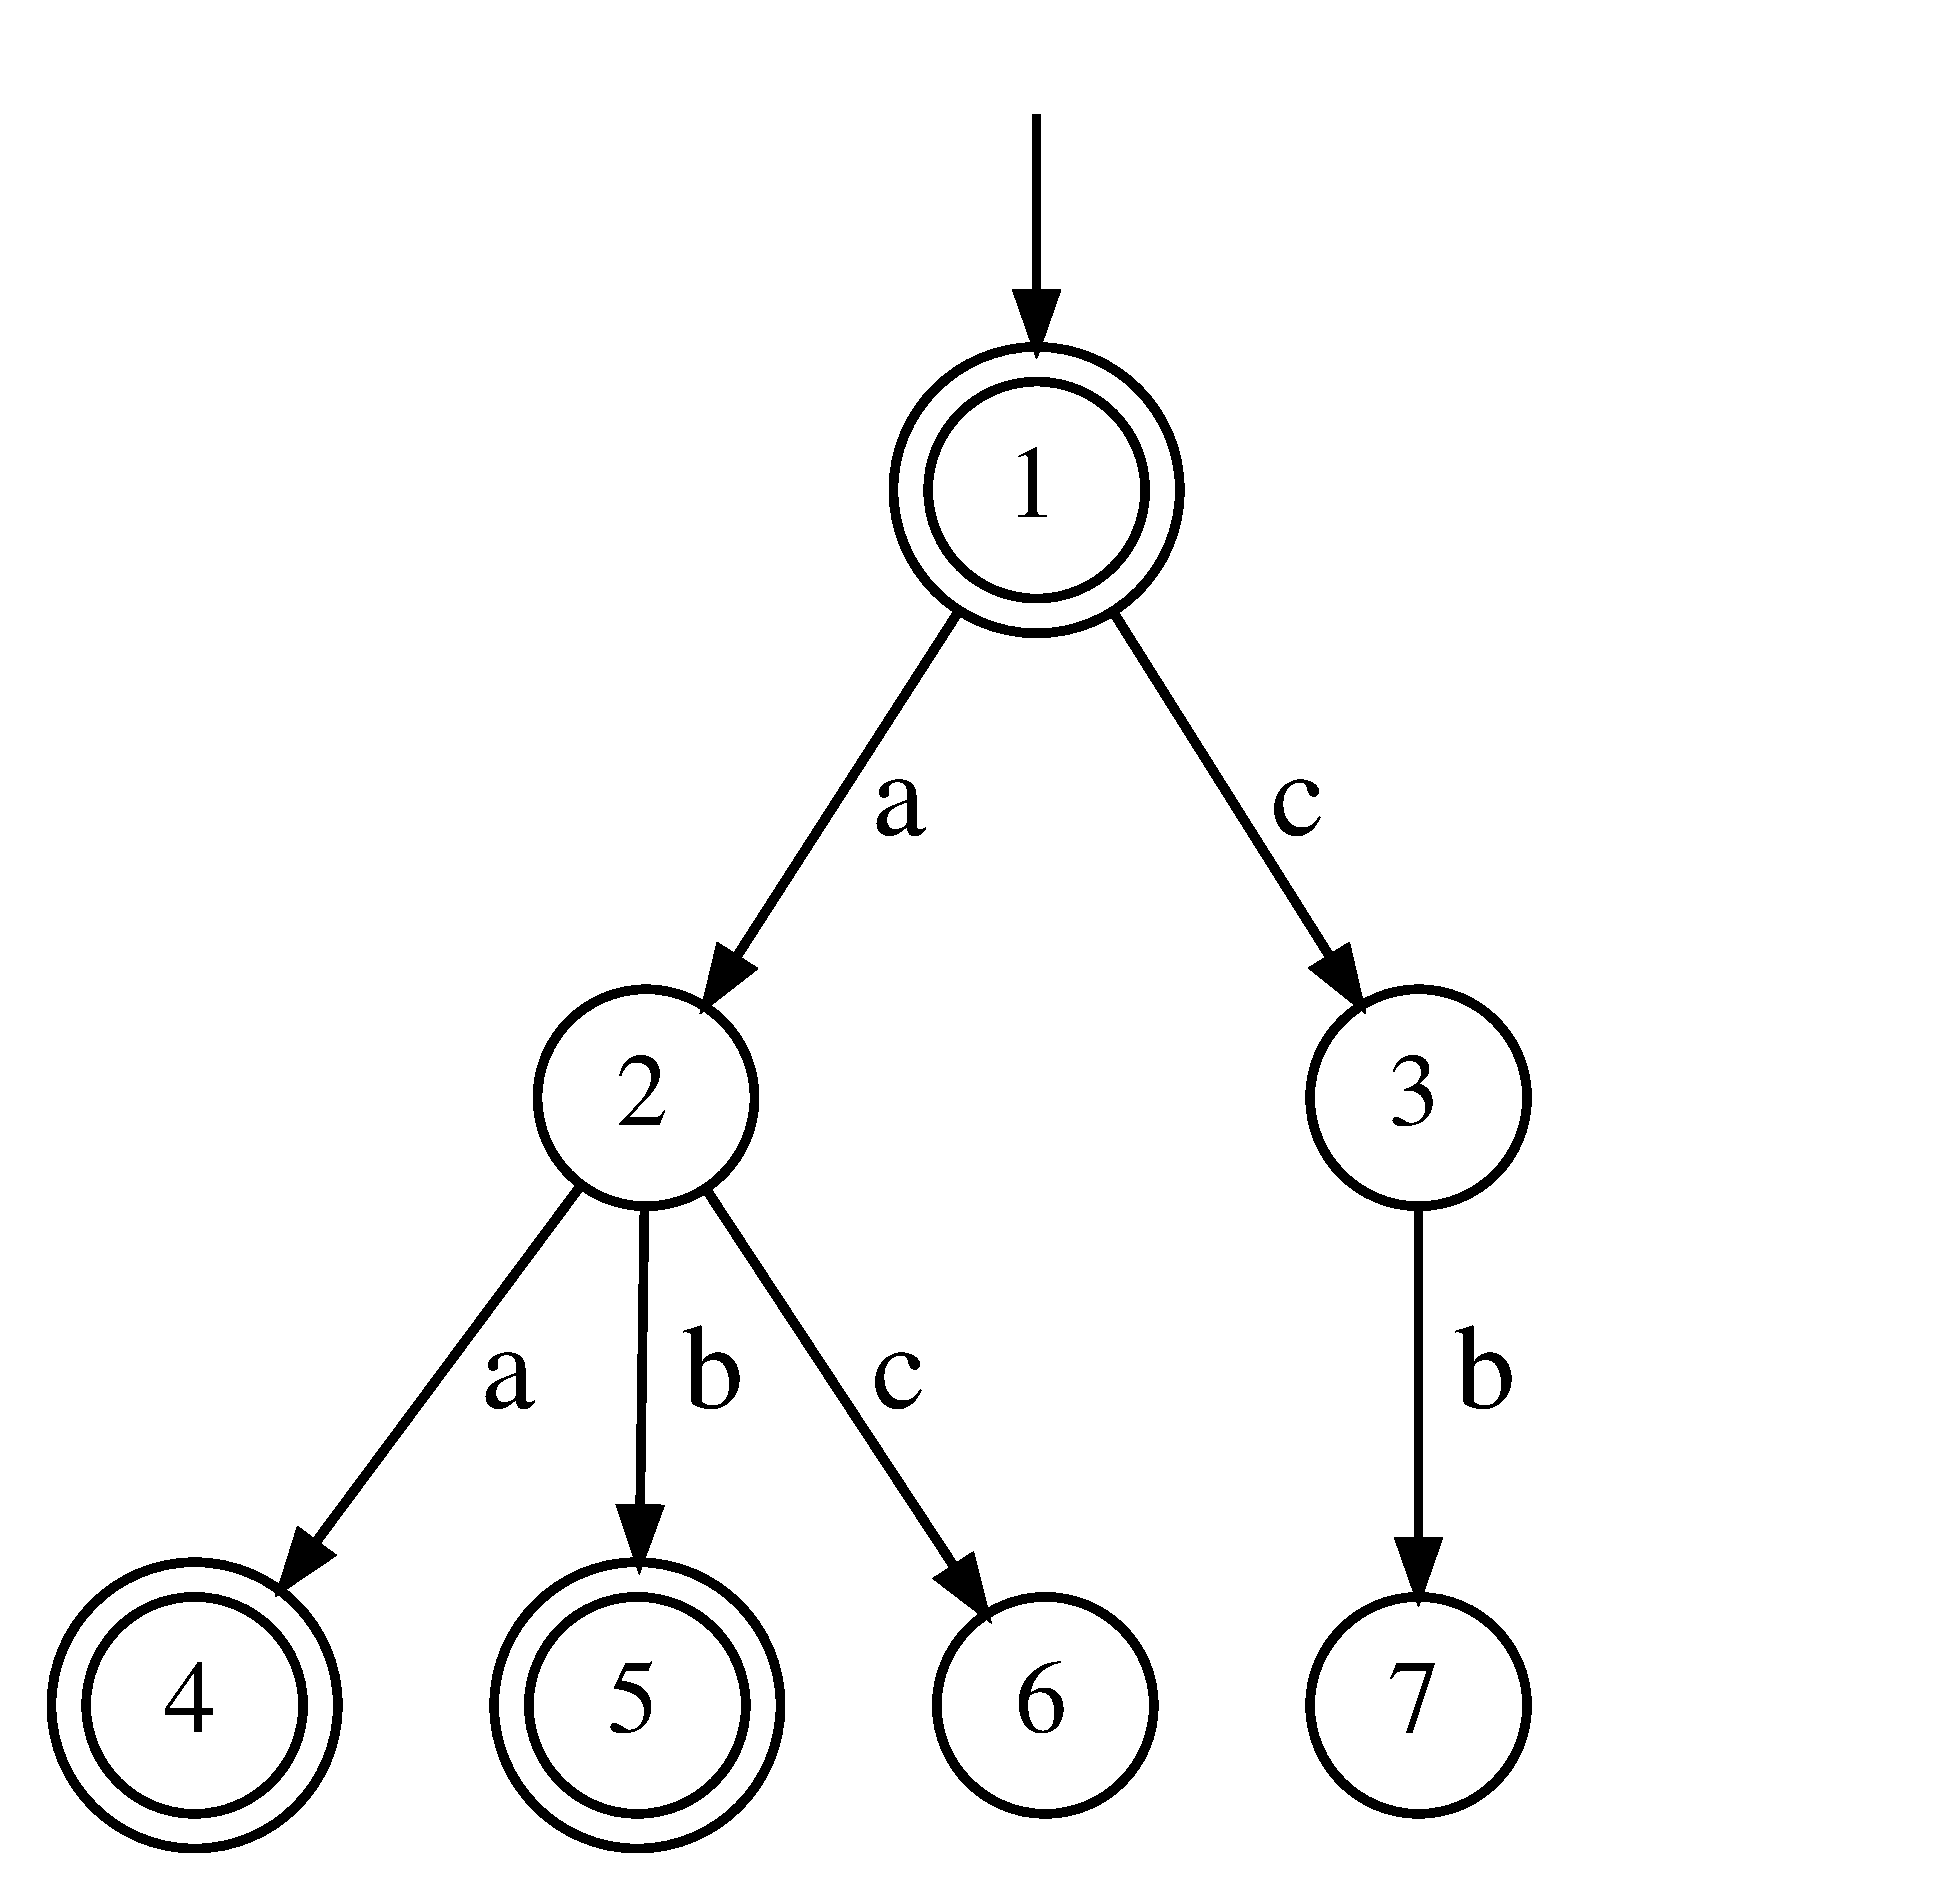
\includegraphics[scale=0.15]{img/datamod/BFS-tree.eps}
    \else
      \begin{tikzpicture}[
    ->, % makes the edges directed
    >=stealth', % makes the arrow heads bold
    node distance=1.7cm, % specifies the minimum distance between two nodes. Change if necessary.
    every state/.style={thick, fill=gray!10, minimum size = 0pt}, % sets the properties for each ’state’ node
    initial text=$ $, % sets the text that appears on the start arrow
]
    \def\xshift{0.53cm}

    \node[state, initial above, accepting] (q1) {$1$};
    \node[state] (q2) [below left of=q1] {$2$};
    \node[state] (q3) [below right of=q1] {$3$};
    \node[state, accepting] (q5) [below of=q2]  {$5$};
    \node[state, accepting] (q4) [left of=q5, xshift=\xshift]  {$4$};
    \node[state] (q6) [right of=q5, xshift=-\xshift]  {$6$};
    \node[state] (q7) [below of=q3]  {$7$};

    \path
        (q1) edge [left] node {a} (q2)
        (q1) edge [right] node {c} (q3)
        (q2) edge [left] node {a} (q4)
        (q2) edge [left] node {b} (q5)
        (q2) edge [right] node {c} (q6)
        (q3) edge [right] node {b} (q7)
        ;
\end{tikzpicture}
    \fi
  }
  \caption{An example of a BFS-enumerated automaton and the corresponding BFS traversal tree}
  \label{syn-en:img:bfs}
\end{figure}

\insectionen{\ref{sec:review:cegar}} the algorithm based on counterexample-guided abstraction refinement (CEGAR) is described.
Methods based on CEGAR are applicable in a situation when one needs to infer a model that corresponds to some given requirements, and a checking system (oracle) is available.
On the first step some model (possibly, random) is constructed.
Then, an iterative process of refining the current model is initiated: on each step the compliance of the current model to the requirements is checked using the oracle.
If the oracle check is successfully passed, then the sought model is found.
Otherwise, the oracle returns one or several counterexamples, which are consequently used to refine the model.

%------

\textbf{\underline{Chapter 2}} describes the development, implementation, and experimental evaluation of DFA inference methods with different approaches to reducing the 
search space during SAT solving.

\insectionen{\ref{sec:space:dfs}} a description of developed symmetry breaking predicates based on encoding the \emph{depth-first search}~(DFS) algorithm is provided.
The use of BFS-based symmetry breaking predicates has previously allowed increasing the efficiency of the \texttt{DFASAT} method considerably.
It was logical to consider as the next research task the development of symmetry breaking predicates based on the DFS algorithm and the method that uses them.
An example of a DFS-enumerated DFA is shown in Figure~\ref{syn-en:img:dfs:dfs-ex}, and~\ref{syn-en:img:dfs:dfs-tree} shows the corresponding traversal tree.

\begin{figure}[ht]
  \centering
  \subfloat[An example of a DFS-enumerated automaton\label{syn-en:img:dfs:dfs-ex}]{
    \ifafour
      % 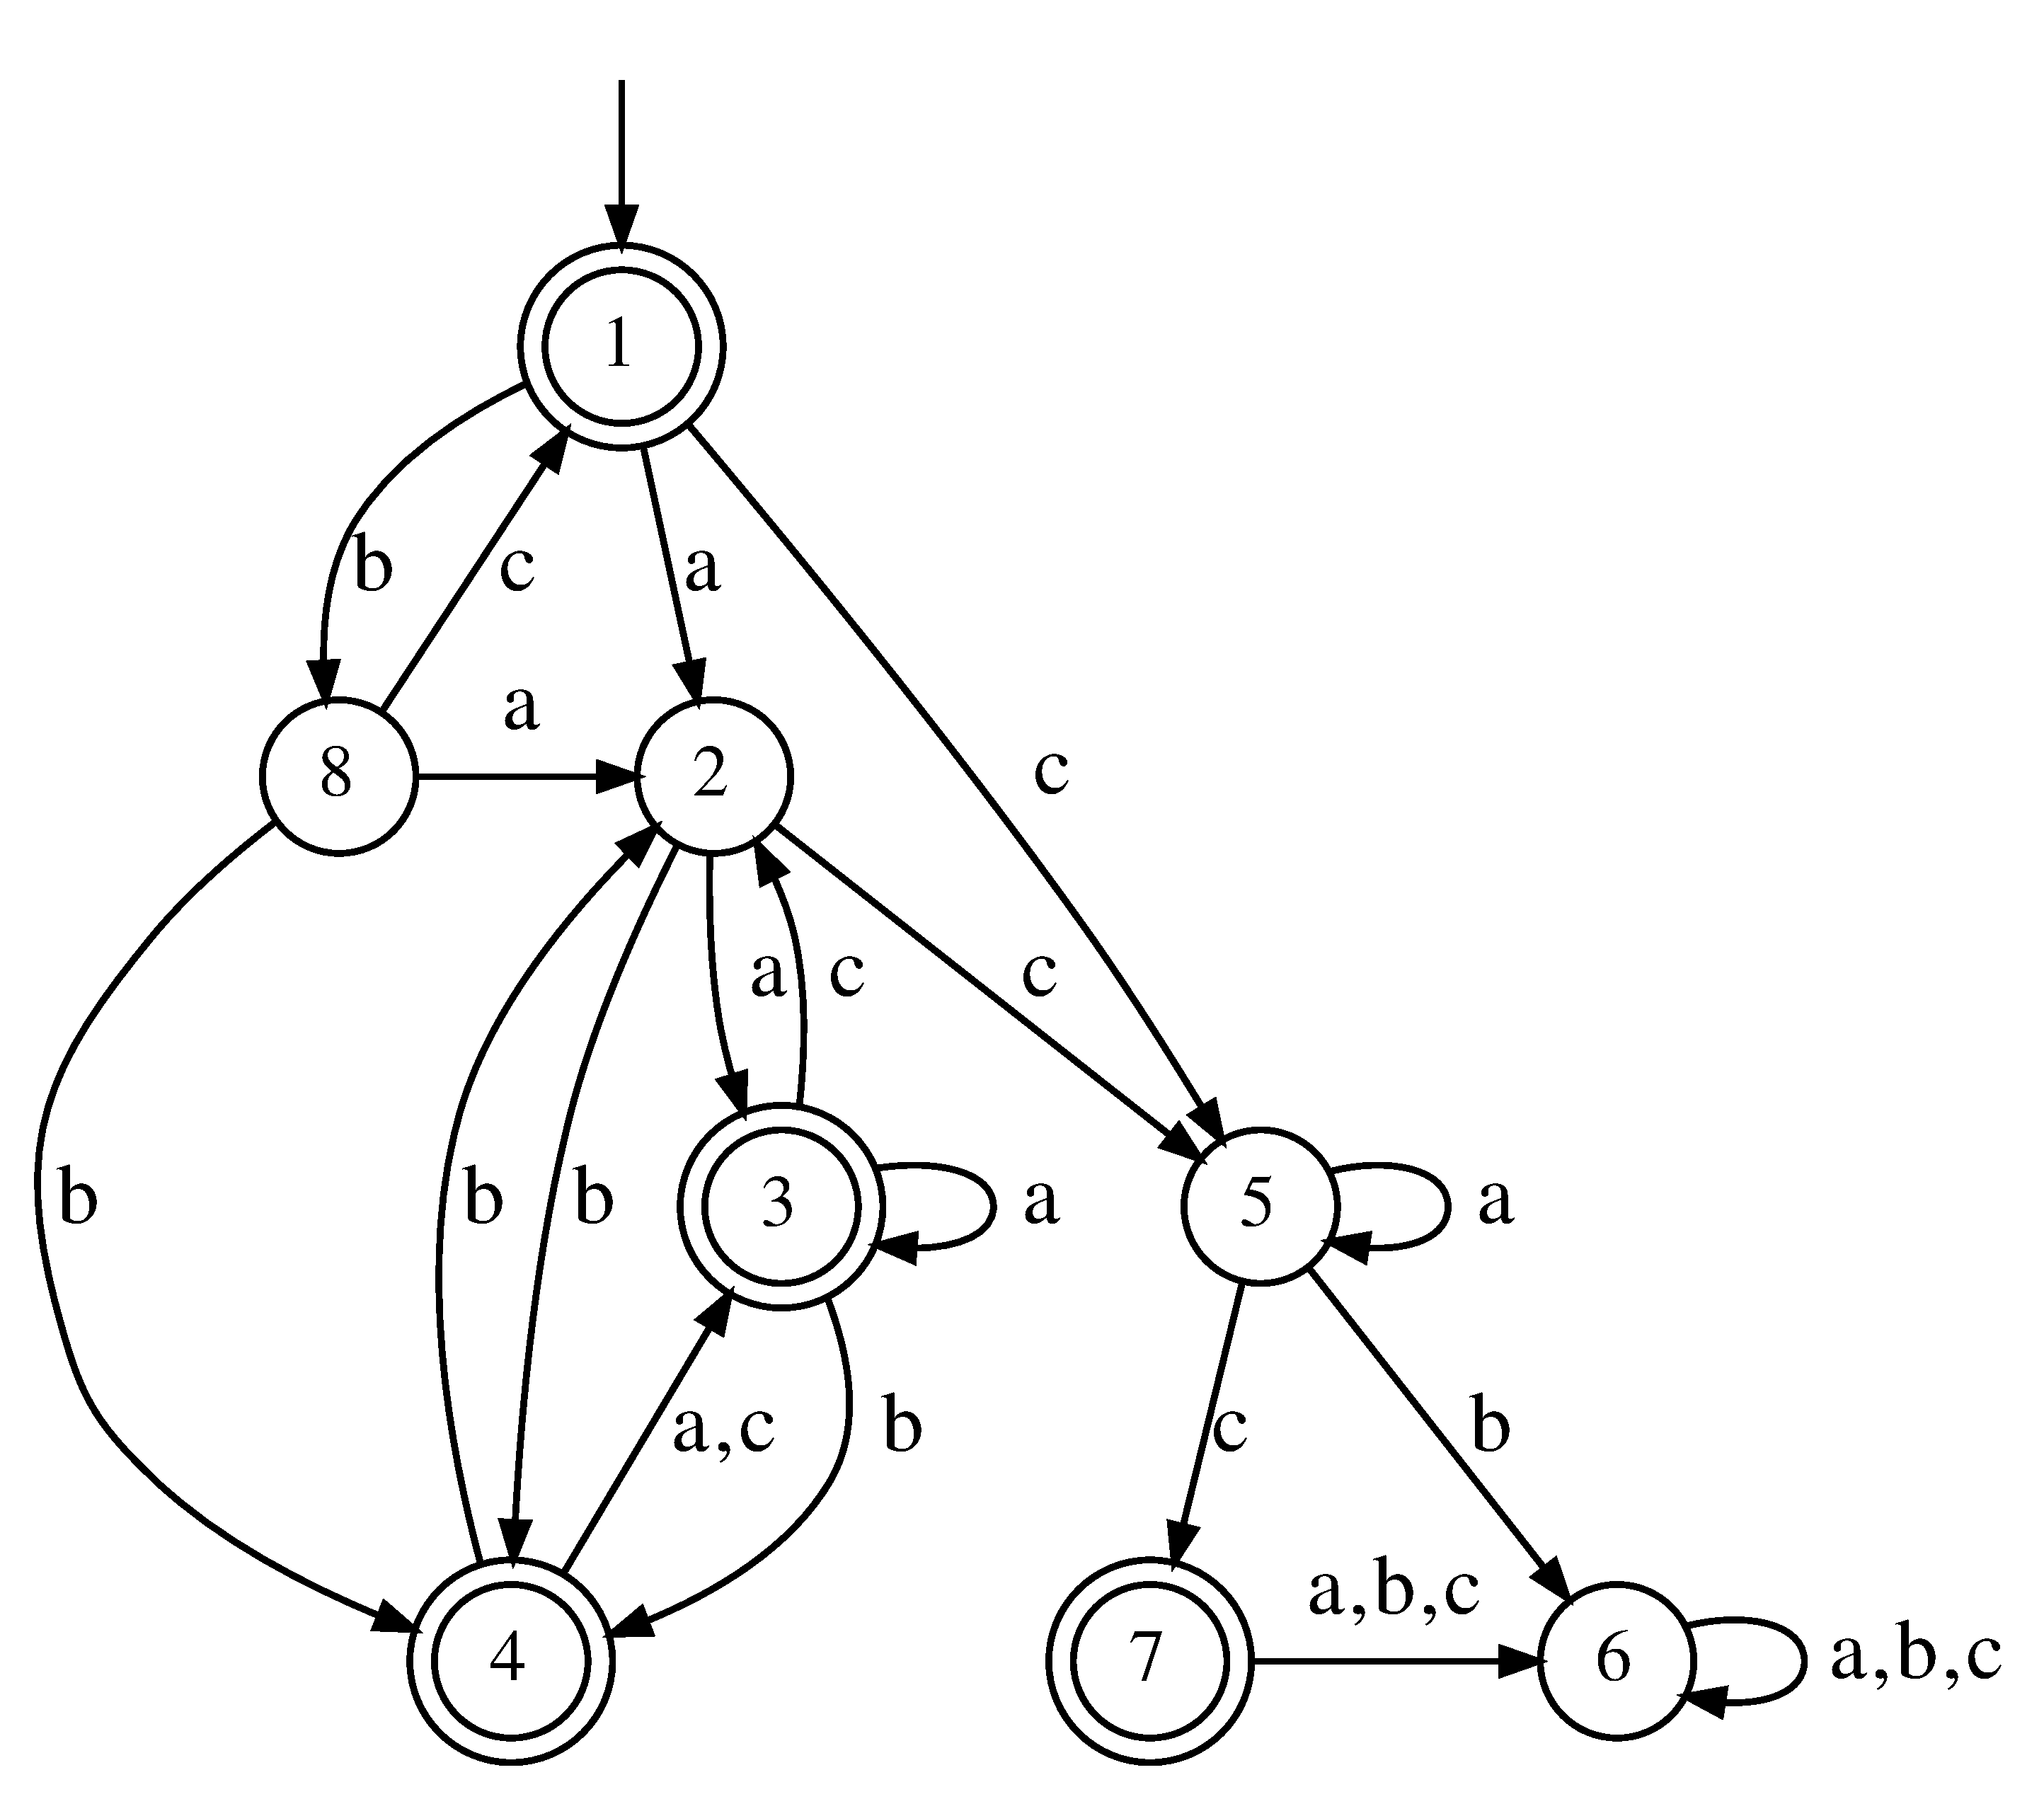
\includegraphics[scale=0.15]{img/datamod/DFS-example.eps}
      \begin{tikzpicture}[
    ->, % makes the edges directed
    >=stealth', % makes the arrow heads bold
    node distance=2.5cm, % specifies the minimum distance between two nodes. Change if necessary.
    every state/.style={thick, fill=gray!10, minimum size = 0pt}, % sets the properties for each ’state’ node
    initial text=$ $, % sets the text that appears on the start arrow
    double distance between line centers=2pt
]
    \node[state, initial above, accepting] (q1) {$1$};
    \node[state] (q2) [below of=q1] {$2$};
    \node[state] (q8) [left of=q2] {$8$};
    \node[state] (q5) [right of=q2] {$5$};
    \node[state, accepting] (q4) [below of=q8] {$4$};
    \node[state, accepting] (q3) [below of=q2] {$3$};
    \node[state, accepting] (q7) [below of=q5] {$7$};
    \node[state] (q6) [right of=q7] {$6$};
    
    \path
        (q1) edge [bend right=10, left] node {b} (q8)
        (q8) edge [bend right=10, right] node {c} (q1)
        (q1) edge [right] node {a} (q2)
        (q1) edge [right] node {c} (q5)
        (q8) edge [above] node {a} (q2)
        (q2) edge [above] node {c} (q5)
        (q3) edge [loop below] node {a} (q3)
        (q5) edge [loop above] node {a} (q5)
        (q6) edge [loop below] node {a,b,c} (q6)
        (q5) edge [right] node {c} (q7)
        (q5) edge [right] node {b} (q6)
        (q7) edge [below] node {a,b,c} (q6)
        (q8) edge [left] node {b} (q4)
        (q4) edge [bend right=10, below] node {a,c} (q3)
        (q3) edge [bend right=10, above] node {b} (q4)
        (q2) edge [bend right=10, left] node {a} (q3)
        (q3) edge [bend right=10, right] node {c} (q2)
        (q4) edge [bend right=10, below] node [xshift=4pt, yshift=4pt] {b} (q2)
        (q2) edge [bend right=10, above] node {b} (q4)
        ;

\end{tikzpicture}
    \else
      \begin{tikzpicture}[
    ->, % makes the edges directed
    >=stealth', % makes the arrow heads bold
    node distance=1.9cm, % specifies the minimum distance between two nodes. Change if necessary.
    every state/.style={thick, fill=gray!10, minimum size = 0pt}, % sets the properties for each ’state’ node
    initial text=$ $, % sets the text that appears on the start arrow
]
    \node[state, initial above, accepting] (q1) {$1$};
    \node[state] (q2) [below of=q1] {$2$};
    \node[state] (q8) [left of=q2] {$8$};
    \node[state] (q5) [right of=q2] {$5$};
    \node[state, accepting] (q4) [below of=q8] {$4$};
    \node[state, accepting] (q3) [below of=q2] {$3$};
    \node[state, accepting] (q7) [below of=q5] {$7$};
    \node[state] (q6) [right of=q7] {$6$};
    
    \path
        (q1) edge [bend right=10, left] node {b} (q8)
        (q8) edge [bend right=10, right] node {c} (q1)
        (q1) edge [right] node {a} (q2)
        (q1) edge [right] node {c} (q5)
        (q8) edge [above] node {a} (q2)
        (q2) edge [above] node {c} (q5)
        (q3) edge [loop below] node {a} (q3)
        (q5) edge [loop above] node {a} (q5)
        (q6) edge [loop below] node {a,b,c} (q6)
        (q5) edge [right] node {c} (q7)
        (q5) edge [right] node {b} (q6)
        (q7) edge [below] node {a,b,c} (q6)
        (q8) edge [left] node {b} (q4)
        (q4) edge [bend right=10, below] node {a,c} (q3)
        (q3) edge [bend right=10, above] node {b} (q4)
        (q2) edge [bend right=10, left] node {a} (q3)
        (q3) edge [bend right=10, right] node {c} (q2)
        (q4) edge [bend right=10, below] node [xshift=2pt, yshift=2pt] {b} (q2)
        (q2) edge [bend right=10, above] node {b} (q4)
        ;

\end{tikzpicture}
    \fi
  }
  \hfill
  \subfloat[The DFS traversal tree for the automaton in Figure~\ref{syn-en:img:dfs:dfs-ex}\label{syn-en:img:dfs:dfs-tree}]{
    \ifafour
      % 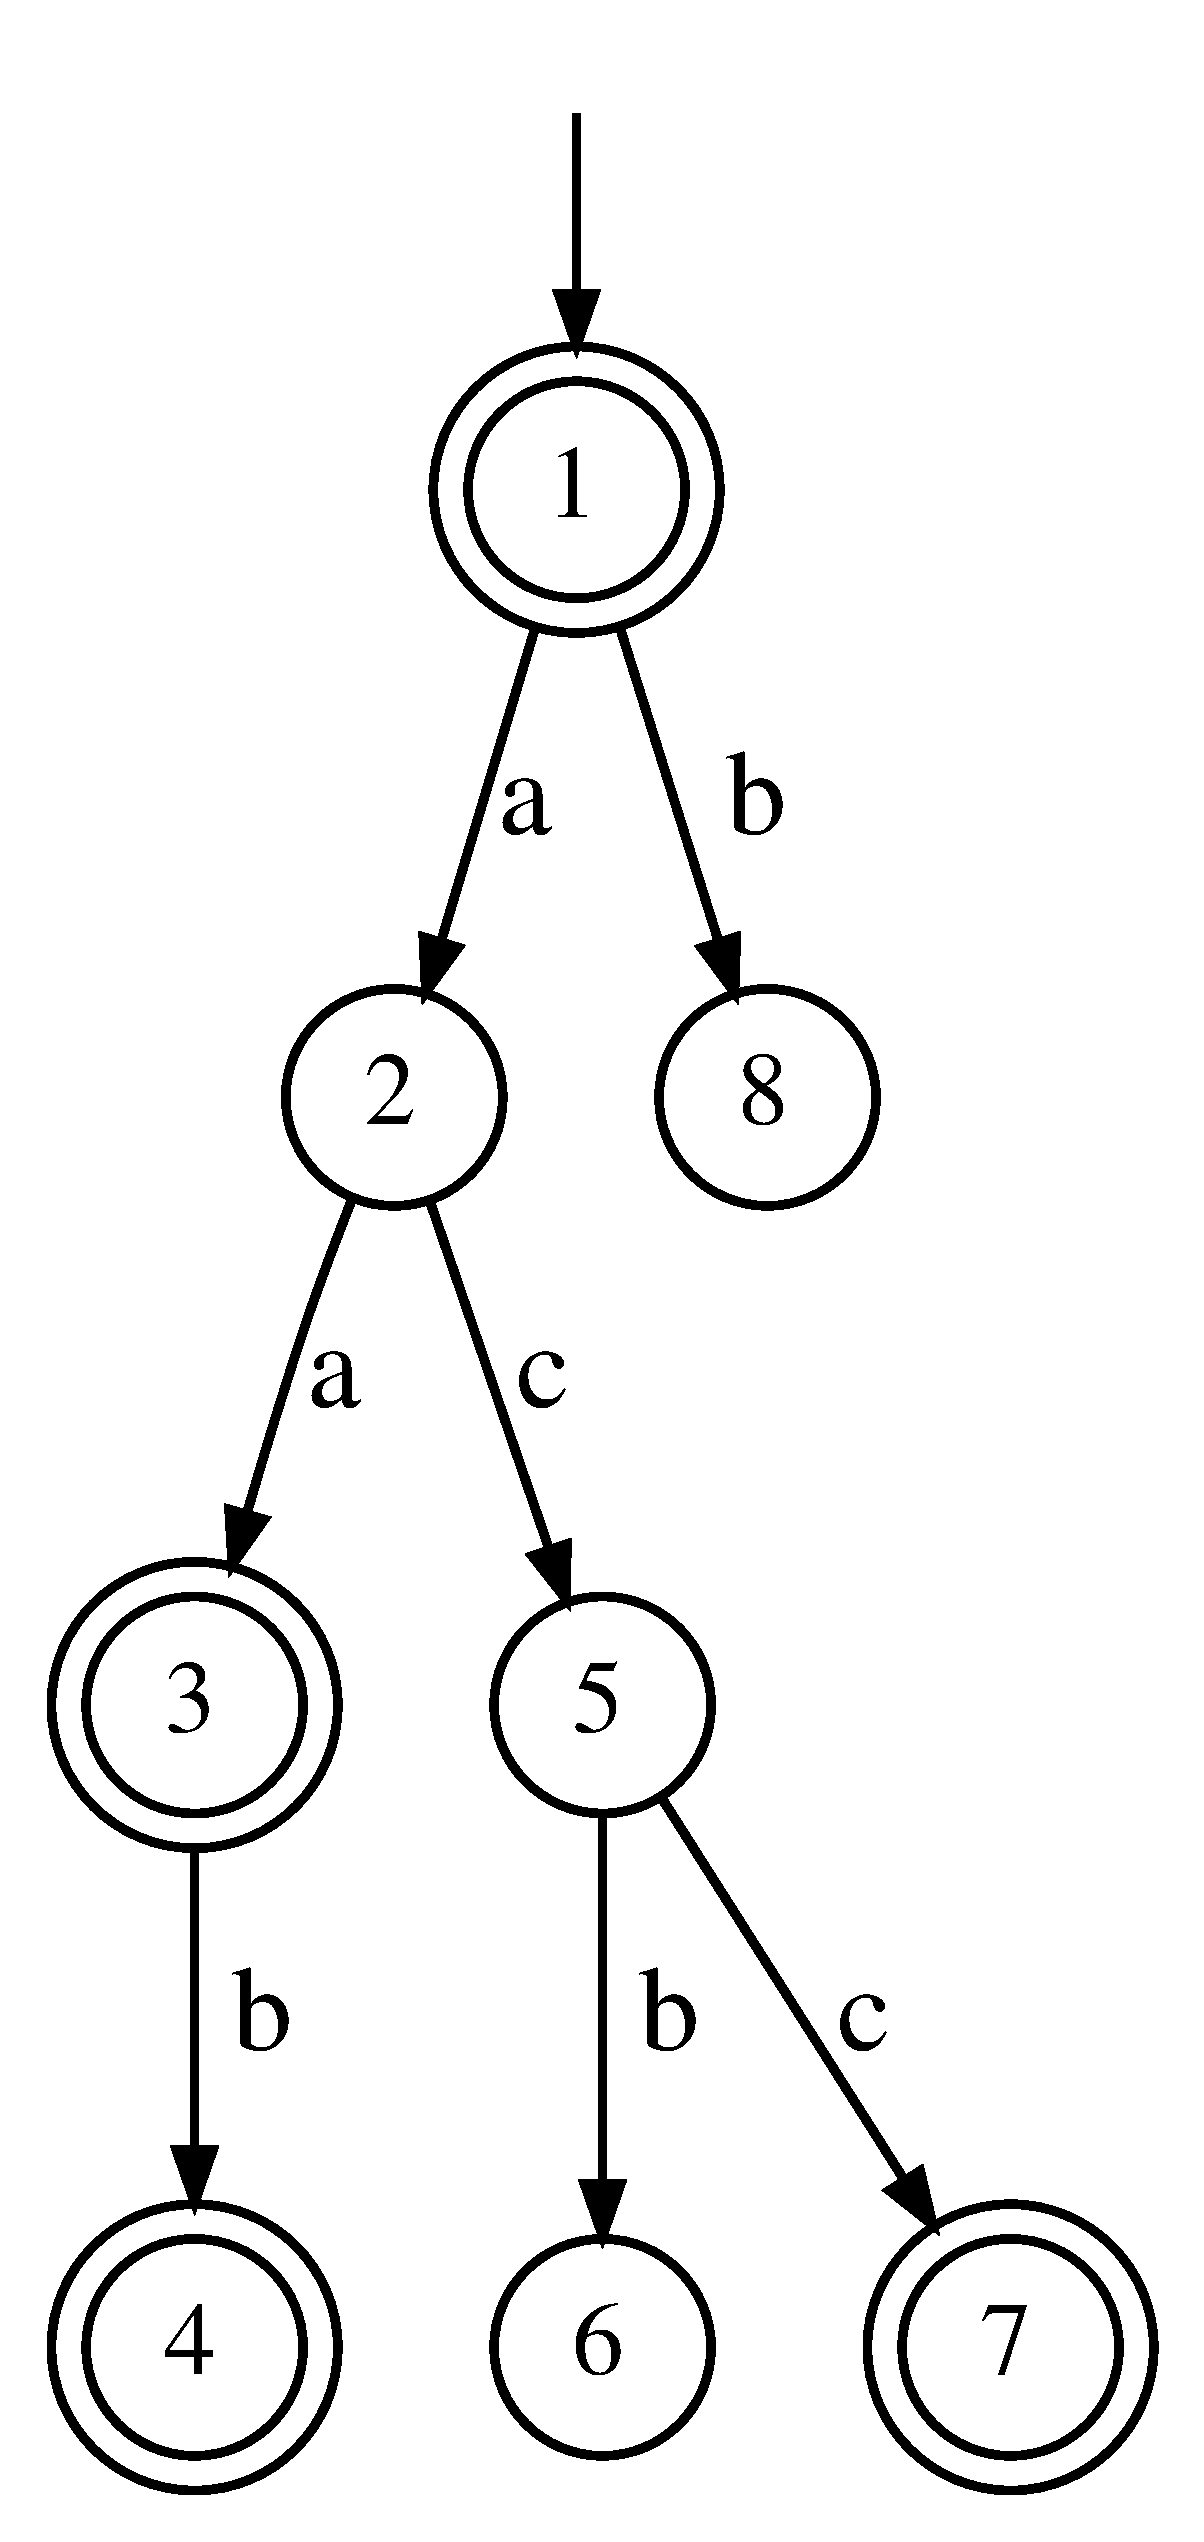
\includegraphics[scale=0.15]{img/datamod/DFS-tree.eps}
      \begin{tikzpicture}[
    ->, % makes the edges directed
    >=stealth', % makes the arrow heads bold
    node distance=2cm, % specifies the minimum distance between two nodes. Change if necessary.
    every state/.style={thick, fill=gray!10, minimum size = 0pt}, % sets the properties for each ’state’ node
    initial text=$ $, % sets the text that appears on the start arrow
    double distance between line centers=2pt
]
    \def\xshift{0.7cm}

    \node[state, initial above, accepting]     (q1)                 {$1$};
    \node[state] (q2) [below of=q1, xshift=-\xshift] {$2$};
    \node[state] (q8) [below of=q1, xshift=\xshift] {$8$};
    \node[state, accepting] (q3) [below of=q2, xshift=-\xshift] {$3$};
    \node[state] (q5) [below of=q2, xshift=\xshift] {$5$};
    \node[state, accepting] (q4) [below of=q3, xshift=-\xshift] {$4$};
    \node[state] (q6) [below of=q5, xshift=-\xshift] {$6$};
    \node[state, accepting] (q7) [below of=q5, xshift=\xshift] {$7$};

    \path
        (q1) edge [left] node {a} (q2)
        (q1) edge [right] node {b} (q8)
        (q2) edge [left] node {a} (q3)
        (q2) edge [right] node {c} (q5)
        (q3) edge [left] node {b} (q4)
        (q5) edge [left] node {b} (q6)
        (q5) edge [right] node {c} (q7)
        ;
\end{tikzpicture}
    \else
      \begin{tikzpicture}[
    ->, % makes the edges directed
    >=stealth', % makes the arrow heads bold
    node distance=1.5cm, % specifies the minimum distance between two nodes. Change if necessary.
    every state/.style={thick, fill=gray!10, minimum size = 0pt}, % sets the properties for each ’state’ node
    initial text=$ $, % sets the text that appears on the start arrow
]
    \def\xshift{0.7cm}

    \node[state, initial above, accepting]     (q1)                 {$1$};
    \node[state] (q2) [below of=q1, xshift=-\xshift] {$2$};
    \node[state] (q8) [below of=q1, xshift=\xshift] {$8$};
    \node[state, accepting] (q3) [below of=q2, xshift=-\xshift] {$3$};
    \node[state] (q5) [below of=q2, xshift=\xshift] {$5$};
    \node[state, accepting] (q4) [below of=q3, xshift=-\xshift] {$4$};
    \node[state] (q6) [below of=q5, xshift=-\xshift] {$6$};
    \node[state, accepting] (q7) [below of=q5, xshift=\xshift] {$7$};

    \path
        (q1) edge [left] node {a} (q2)
        (q1) edge [right] node {b} (q8)
        (q2) edge [left] node {a} (q3)
        (q2) edge [right] node {c} (q5)
        (q3) edge [left] node {b} (q4)
        (q5) edge [left] node {b} (q6)
        (q5) edge [right] node {c} (q7)
        ;
\end{tikzpicture}
    \fi
  }
  \caption{An example of a DFS-enumerated automaton and the corresponding DFS-traversal tree}
  \label{syn-en:img:dfs}
\end{figure}

The developed predicates are expressed as a CNF formula with $\mathcal{O}\left(M^{4} + M^{3} \times L^{2}\right)$ clauses, 
which is $M$ times greater than the number of clauses for the BFS-based DFA symmetry breaking predicates.

\insectionen{\ref{sec:space:tight}} a description of the developed compact BFS-based symmetry breaking predicates is given.

The compactness of the developed predicates consists in reduction of the size of the formula that encodes the BFS-based symmetry breaking predicates from
$\mathcal{O}\left(M^{3} + M^{2} \times L^{2}\right)$ to $\mathcal{O}\left(M^{2} \times L\right)$ clauses.
Analysis of constraints from the original encoding, which were expressed using $\mathcal{O}\left(M^{3}\right)$ и $\mathcal{O}\left(M^{2} \times L^{2}\right)$ clauses,
showed that some parameters that define the size of the formula are independent, and other parameters may be eliminated by introduction of new variables.
For each such constraint a way of making it more compact was developed, leading to an overall decrease of formula size.
Apart from this, the majority of clauses for the original encoding, which consisted of  $\mathcal{O}\left(M\right)$ literals,
were replaced by clauses comprised of two or three literals: this considerably influences the performance of SAT solvers, since such clauses are processed in constant time
and are not stored in memory~\cite{MSilva-SATbook09}.

\textbf{Section~\ref{sec:space:pruning}} describes developed search space reduction approaches for DFA inference, that are based on BFS tree structure properties, 
also on connections between the augmented prefix tree acceptor and the sought DFA.
Figure~\ref{syn-en:img:full-bfs} shows a complete BFS tree of an arbitrary size on an arbitrary $L$-sized alphabet.
The tree is called complete since each vertex has exactly $L$ children.

\begin{figure}[ht]
  \centering
  \scalebox{0.625}{%
\begin{tikzpicture}[scale=0.75, level 1/.style={sibling distance=60mm},level 2/.style={sibling distance=40mm}, level distance=25mm, level 3/.style={sibling distance=50mm}]
\node [ellipse,draw] (root){$1$}
  child {node [ellipse,draw] (a0) {$2$}
    child {node [ellipse,draw] (a0b0) {$L+2$}}
    child {node [ellipse,draw] (a0bj) {$L+j+1$}}
    child {node [ellipse,draw] (a0bL) {$2L+1$}}
  }
  child {node (aj) {$\vdots$}
    child {node [ellipse,draw] (r) {$r$}
      child {node [xshift=-0.25em,ellipse,draw] (r0) {$(r-1)L+2$}}
      child {node [ellipse,draw] (rj) {$(r-1)L+j+1$}}
      child {node [xshift=0.25em,ellipse,draw] (rL) {$rL+1$}}
    }
  }
  child {node [ellipse,draw] (aL) {$L+1$}
    child {node [ellipse,draw] (aLb0) {$L^2+2$}}
    child {node [ellipse,draw] (aLbj) {$L^2+j+1$}}
    child {node [ellipse,draw] (aLbL) {$L^2+L+1$}}
  }
;

\path (root) -- (a0) node [below, midway, darkblue] {$1$};
\path (root) -- (aL) node [below, midway, darkblue] {$L$};

\path (a0) -- (a0b0) node [below, midway, darkblue] {$1$};
\path (a0) -- (a0bj) node [left, midway, darkblue] {$j$};
\path (a0) -- (a0bL) node [below, midway, darkblue] {$L$};

\path (aL) -- (aLb0) node [below, midway, darkblue] {$1$};
\path (aL) -- (aLbj) node [left, midway, darkblue] {$j$};
\path (aL) -- (aLbL) node [below, midway, darkblue] {$L$};

\path (r) -- (r0) node [below, midway, darkblue] {$1$};
\path (r) -- (rj) node [left, midway, darkblue] {$j$};
\path (r) -- (rL) node [below, midway, darkblue] {$L$};

\path (a0) -- (aj) node [midway] {$..$};
\path (aj) -- (aL) node [midway] {$..$};

\path (a0b0) -- (a0bj) node [midway] {$..$};
\path (a0bj) -- (a0bL) node [midway] {$..$};

\path (aLb0) -- (aLbj) node [midway] {$..$};
\path (aLbj) -- (aLbL) node [midway] {$..$};

\path (r0) -- (rj) node [midway] {$..$};
\path (rj) -- (rL) node [midway] {$..$};
\end{tikzpicture}
%
%
\begin{comment}
%
%
\begin{figure}
\centering
\begin{tikzpicture}[scale=0.75, level 1/.style={sibling distance=60mm},level 2/.style={sibling distance=40mm}, level distance=25mm, level 3/.style={sibling distance=50mm}]
\node [ellipse,draw] (root){$1$}
  child {node [ellipse,draw] (a0) {$2$}
   child {node [ellipse,draw] (a0b0) {$L+2$}}
   child {node [ellipse,draw] (a0bj) {$L+j+2$}}
   child {node [ellipse,draw] (a0bL) {$2L+1$}}
  }
  child {node (aj) {$\vdots$}
    child {node [ellipse,draw] (r) {$r$}
      child {node [ellipse,draw] (r0) {$(r-1)L+2$}}
      child {node [ellipse,draw] (rj) {$(r-1)L+j+2$}}
      child {node [ellipse,draw] (rL) {$rL+1$}
        child [grow=right,red] {node [red] (j) {$0\leq j < L$} edge from parent[draw=none]}
      }
    }
  }
  child {node [ellipse,draw] (aL) {$L+1$}
    child {node [ellipse,draw] (aLb0) {$L^2+2$}}
    child {node [ellipse,draw] (aLbj) {$L^2+j+2$}}
    child {node [ellipse,draw] (aLbL) {$L^2+L+1$}}
  }
;

\path (root) -- (a0) node [midway, red] {$0$};
\path (root) -- (aL) node [midway, red] {$L-1$};

\path (a0) -- (a0b0) node [midway, red] {$0$};
\path (a0) -- (a0bj) node [midway, red] {$j$};
\path (a0) -- (a0bL) node [midway, red] {$L-1$};

\path (aL) -- (aLb0) node [midway, red] {$0$};
\path (aL) -- (aLbj) node [midway, red] {$j$};
\path (aL) -- (aLbL) node [midway, red] {$L-1$};

\path (r) -- (r0) node [midway, red] {$0$};
\path (r) -- (rj) node [midway, red] {$j$};
\path (r) -- (rL) node [midway, red] {$L-1$};

\path (a0) -- (aj) node [midway] {$..$};
\path (aj) -- (aL) node [midway] {$..$};

\path (a0b0) -- (a0bj) node [midway] {$..$};
\path (a0bj) -- (a0bL) node [midway] {$..$};

\path (aLb0) -- (aLbj) node [midway] {$..$};
\path (aLbj) -- (aLbL) node [midway] {$..$};

\path (r0) -- (rj) node [midway] {$..$};
\path (rj) -- (rL) node [midway] {$..$};
\end{tikzpicture}
\caption{Worst case BFS tree with $0\leq j <L$}
\end{figure}
%
%
\end{comment}
}
  \caption{A complete BFS tree with $\abs{\Sigma}=L$}
  \label{syn-en:img:full-bfs}
\end{figure}

Following an analysis of this tree some properties and constraints that are characteristic for a BFS tree were formulated.
For example, it has been proved that for a vertex with index $r$ in the complete tree, its rightmost child has index $rL + 1$.
Furthermore, we proved that then $rL + 1$ is the upper bound for the index of vertex $r$ in an arbitrary BFS tree.
Then we can state that in an arbitrary BFS tree a vertex with index $n$ can only have children with indices from the range from $r + 1$ to $rL + 1$.
Introduction of these constraints allows reducing the number variables used in the encoding and thus reduce this size of the resulting formula.

By definition, in any BFS tree the children of any vertex $r$ have consecutive indices, and there are no more than $L$ children.
We analyzed the connection between vertices of the APTA vertices and the DFA states.
If the prefix tree contains a path of length $k$ from the root to some vertex $t_{i}$, and vertex $t_{i}$ corresponds to state $d_{j}$ of the sought automaton, then
the automaton must contain a path of length no more than $k$ from the initial state to state $d_{j}$.
A SAT encoding of these properties was developed.
Augmentation of the formula with corresponding constraints allows for additional reduction of the search space during SAT solving.

\textbf{Section{\ref{sec:space:results}}} describes the developed software tool \texttt{DFA-Inductor-py} for DFA inference, implementation of developed methods as parts of 
this software tool, and results of experimental evaluation of all developed methods.

In the process of preparing this thesis a software tool \texttt{DFA-Inductor-py}~\cite{dfa-inductor-py-en} for DFA inference from behavior examples has been developed using the 
\emph{Python} programming language.
The tool is comprised of various modules for solving the problem of DFA inference from behavior examples, the problem of DFA inference from an excessive set of 
behavior examples, and the problem of inferring all non-isomorphic DFA from given behavior examples~(these methods are described in the following chapters).
The tool implements different symmetry breaking predicates, including ones previously proposed by other authors, and the ones developed in this thesis.

The developed software tool was used to perform two series of experimental evaluations.
First we compared two methods for DFA inference from behavior examples that use symmetry breaking predicates based on BFS and DFS, correspondingly.
Since these two methods are based on the method \texttt{DFASAT}, in which symmetry breaking constraints are based on fixing the enumeration of some large clique in the consistency graph, we also added \texttt{DFASAT} to this experimental evaluation.

Publicly open tests (sets of behavior examples), for example, from \emph{Abbadingo One DFA Learning Competition}~\cite{DBLP:conf/icgi/LangPP98} and \emph{StaMinA Competition}~\cite{DBLP:journals/ese/WalkinshawLDBD13}, were developed for inexact algorithms which can generate automata with hundreds of states.
Exact methods, both existing and proposed in this thesis, are currently not capable of inferring DFA of such size; for this reason, tests for this experimental evaluation
were generated randomly.
Experimental results are shown in Table~\ref{syn-en:tab:DFS-results} and allow drawing the conclusion that the use of DFS-based symmetry breaking predicates is impractical,
since the method that uses them is significantly inferior to the method that uses BFS-predicates.
However, note that the method that uses DFS-predicates still considerably outperforms \texttt{DFASAT}.
Nevertheless, based on experimental results, it was decided not to continue the development of DFS-predicates and concentrate on improving predicates based on the 
breadth-first search algorithm.

\begin{table}[ht]
  \caption{Median execution time in seconds for methods of DFA inference from behavior examples: method based on BFS symmetry breaking predicates, based on DFS symmetry breaking predicates, and the \texttt{DFASAT} method. Each value was calculated as a result of 100 independent runs on 100 problems. The execution of the methods was limited to one hour ($\text{TL} = 3600\,\, \text{seconds}$)}
  \centering
  \scalebox{0.95}{
    \begin{tabular}{cccccc}
      M & DFS     & & BFS    & & \texttt{DFASAT}\\
      \hline
      10 & 20.9   & & 20.5   & & 23.3  \\
      12 & 40.4   & & 37.6   & & 240.3 \\
      14 & 82.2   & & 62.4   & & ---   \\
      16 & 205.1  & & 114.1  & & ---   \\
      18 & 601.7  & & 181.9  & & ---   \\
      20 & 2501.6 & & 293.7  & & ---   \\
      22 & ---    & & 453.3  & & ---   \\
      24 & ---    & & 625.1  & & ---   \\
      26 & ---    & & 925.8  & & ---   \\
      28 & ---    & & 1314.4 & & ---   \\
      30 & ---    & & 1635.5 & & ---   \\
    \end{tabular}
  }
  \label{syn-en:tab:DFS-results}
\end{table}

In the second experimental evaluation we compared methods that use the original BFS-predicates (\texttt{DFA-Inductor}) and the BFS-predicates proposed in this thesis (\texttt{DFA-Inductor-py}).
As before, we also considered \texttt{DFASAT} and used randomly generated tests.
Comparison results of all three methods are depicted in Figure~\ref{syn-en:img:plots:cactus} and show that within a fixed time budget \texttt{DFA-Inductor-py} can solve more instances of the problem of DFA inference from behavior examples than \texttt{DFA-Inductor}: in ten minutes the new method solved 731 solved problems against 678 for the old one.
Also note that \texttt{DFASAT} cannot compete with two other methods.

Figure~\ref{syn-en:img:plots:scatter} depicts a more detailed compaison of \texttt{DFA-Inductor} и \texttt{DFA-Inductor-py}: one may notice that the method proposed in this thesis
shows better results for the vast majority of instances.

\begin{figure}[ht]
  \centering
  \begin{subfigure}[b]{0.48\textwidth}
    \centering
    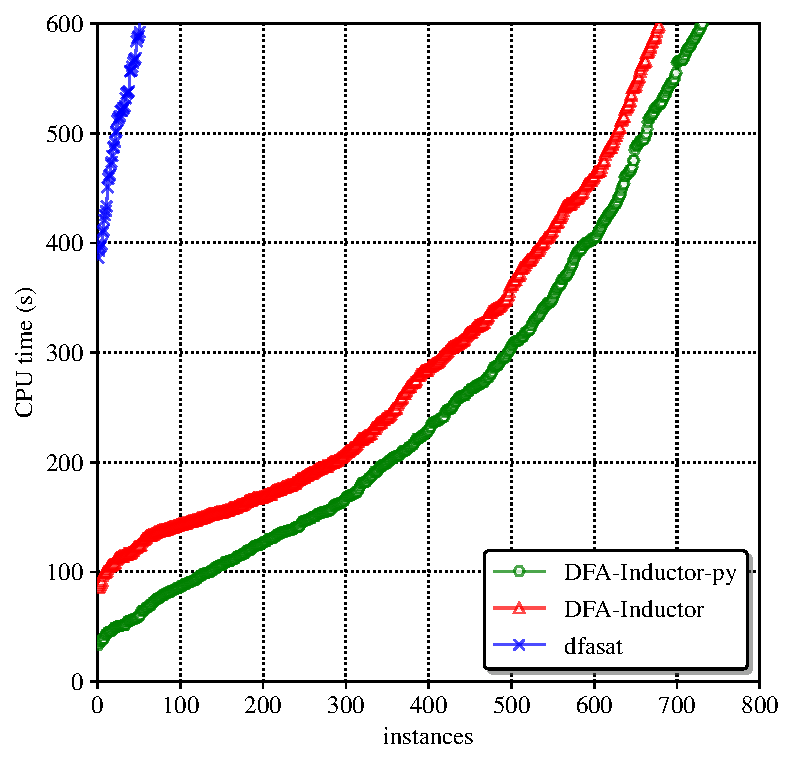
\includegraphics[width=\textwidth]{img/lata19/plots/cactus}
    \caption{Comparison of methods \texttt{DFA-Inductor}, \texttt{DFA-Inductor-py}, and \texttt{DFASAT}, showing the number of problem instances solved within a fixed time budget}
    \label{syn-en:img:plots:cactus}
  \end{subfigure}%
  \;\;
  \begin{subfigure}[b]{0.48\textwidth}
    \centering
    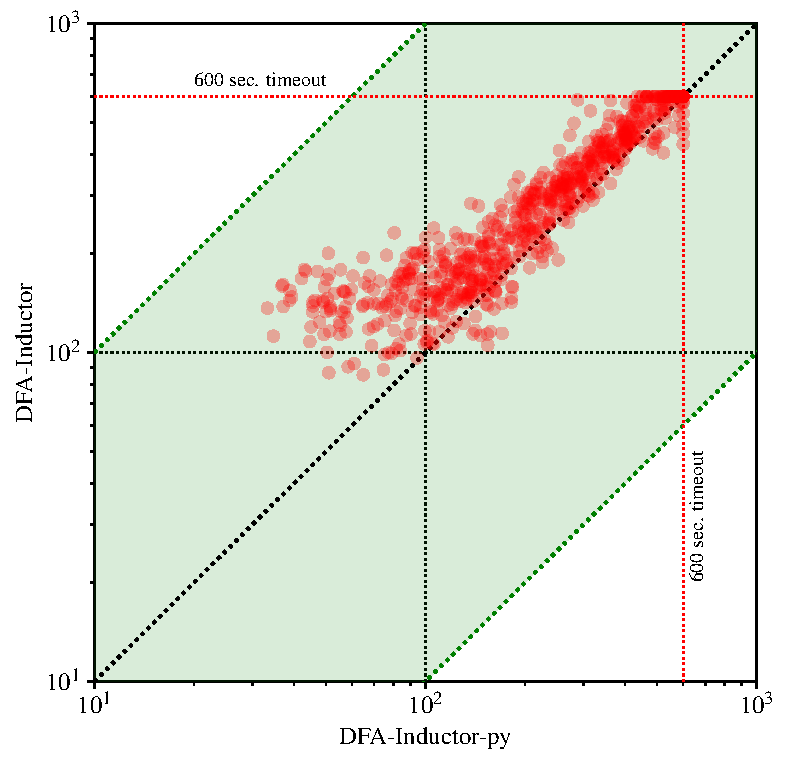
\includegraphics[width=\textwidth]{img/lata19/plots/scatter}
    \caption{Detailed comparison of methods \texttt{DFA-Inductor} and \texttt{DFA-Inductor-py}, showing their performance for each problem instance}
    \label{syn-en:img:plots:scatter}
  \end{subfigure}
  \caption{Comparison results of the method that uses the original BFS-predicates (\texttt{DFA-Inductor}), the method that uses new BFS-predicates (\texttt{DFA-Inductor-py}), and \texttt{DFASAT}}
  \label{syn-en:img:plots}
\end{figure}

%------

\textbf{\underline{Chapter 3}} describes the development, implementation, and experimental evaluation of the exact method for DFA inference from an excessive set of behavior
examples using a reduction to SAT and counterexample-guided abstraction refinement.

\insectionen{\ref{sec:cegar:motivation}} we provide the study of the limits of applicability of methods proposed in previous chapters in dependence on the size of the augmented
prefix tree acceptor.
The size of the Boolean formula that encodes the DFA inference problem depends linearly on the size of the prefix tree:
$\mathcal{O}\left(N \times M^{2}\right)$ clauses, where $N$ is the size of the prefix tree and $M$ is the size of the DFA.
The number of variables in the Boolean formula also linearly depends on the size of the prefix tree: $\mathcal{O}\left(N \times M + M^{2}\right)$ variables.
Thus, when the sought automaton is fixed, the size of the Boolean formula and the number of its variables may vary considerably depending on the number of behavior examples and
their length.
As the size of the prefix tree increases, the SAT solver has to use more and more resources to store the formula and handle it, and the number of variables also increases.
This leads to a situation when the same automaton may be constructed by a SAT solver in seconds from a small set of behavior examples, and may not be found in hours and days in 
the case of an excessive number of long behavior examples.

Since in the case of DFA the key information about each behavior example (whether this word is accepted by the DFA) is contained in the last vertex of a path in the APTA corresponding to this word, it is doubtful that anything can be done in the case of long behavior examples.
However, in the case of an excessive number of behavior examples we can take only a subset of them and infer the same automaton faster.
The issue is in the way the behavior examples are selected: it is possible to accidently eliminate the examples that are necessary to generate the DFA that is the answer to the original problem,
and thus end up with a completely different DFA.
The next section proposes a method that solves this problem: it iteratively enumerates meaningful behavior examples from the original set.

\textbf{Section~\ref{sec:cegar:cegar-algo}} describes the proposed exact method for DFA inference from an excessive set of behavior examples, that is based on a reduction 
to SAT and the CEGAR approach.
As noted before, counterexample-guided abstraction refinement is commonly used in active learning problems.
The considered problem of DFA inference is, on the contrary, a passive learning problem.
However, in this thesis a method is proposed that solves the problem of DFA inference from behavior examples using ideas of the CEGAR approach.

Similar to the classical CEGAR, the proposed approach iteratively refines the model, which in this thesis is a deterministic finite automaton.
The initial prefix tree does not contain any vertices, but is augmented on each step.
On each step it is proposed to try inferring a DFA of the current size for the current prefix tree using a reduction to SAT.
If such a DFA does not exist, then, as before, the size of the sought DFA is increased by one, and the search process is repeated.
And if such an automaton is found, its compliance with the remaining behavior examples is checked.
If the DFA complies with all behavior examples, then the problem is solved.
If not, then we select one or several counterexamples from the behavior examples which are not safisfied by the DFA, and use them to augment the prefix tree,
build a new Boolean formula, and continue the search.
The scheme of the proposed method is shown in Figure~\ref{syn-en:img:cegar-algo}.

\begin{figure}[ht]
  \centering
  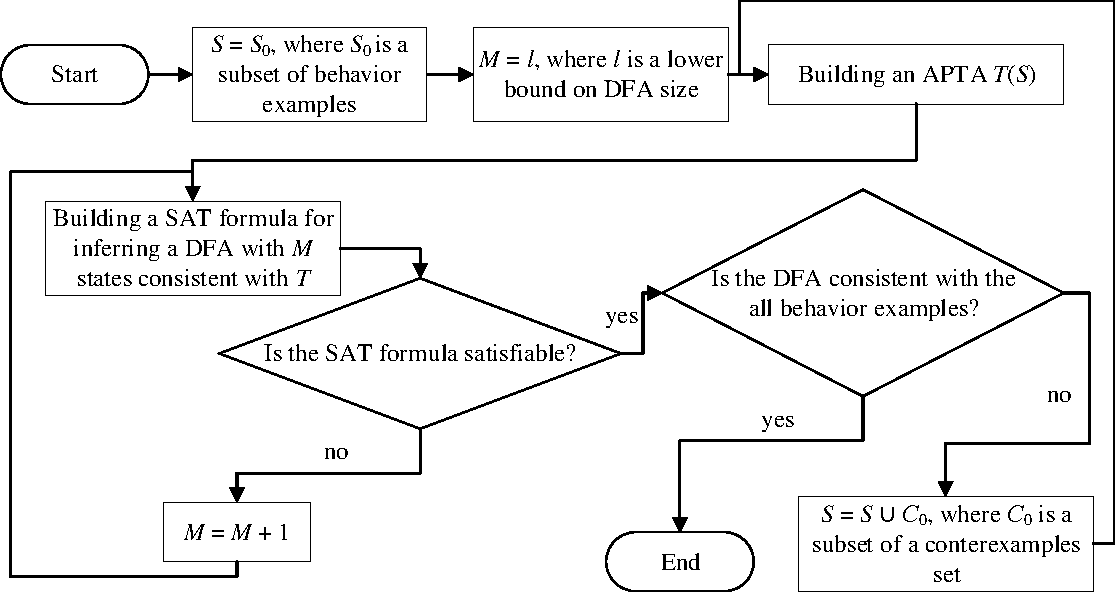
\includegraphics[scale=0.85]{img/ntv/cegar-en.pdf}
  \caption{Scheme of the exact method for DFA inference from an excessive set of behavior examples based on a reduction to SAT and the CEGAR approach}
  \label{syn-en:img:cegar-algo}
\end{figure}

Note that restarting the SAT solver after each augmentation of the prefix tree is extremely inefficient, since when new clauses are added to the formula, 
the search space of SAT is only reduced, and thus, there is no fundamental need to start searching for a satisfying assignment from scratch.
Incremental SAT solvers may be used to cope with this: after some satisfying assignment is found they switch to a state in which they wait for new clauses to be supplied,
and continue the search with a new refined formula from the same place where the search was paused before.


\textbf{Section~\ref{sec:cegar:results}} presents a description of the implementation of the developed method as a part of the tool \texttt{DFA-Inductor-py}, 
as well as results of experimental evaluation of the developed method.
In experimental evaluation we again used random tests.
Results of experimental evaluation showed that when the size of behavior examples $S=\abs{S_{+}}+\abs{S_{-}}$ exceeds $200 \times M$,
the CEGAR-based method works at least two times faster than the method that uses all behavior examples at once.
Moreover, the benefit of using CEGAR increases with the growth of the number of behavior examples.

%------

In \textbf{\underline{Chapter 4}} the problem of inferring all non-isomorphic DFA from given behavior examples is formulated, and the development, implementation, and
experimental evaluation of two methods that solve this problem is described.

\textbf{Section~\ref{sec:findall:problem}} provides a formal statement of the problem of inferring all non-isomorphic DFA of minimal size that satisfy given behavior examples.
As shown before, a DFA of minimal size yields a maximally exact generalization of given data expressed with behavior examples.
However, in the case when the behavior examples do not describe the sought automaton to a satisfactory degree, several different and minimal non-isomorphic automata may exist.
In this case a rational solution may be to infer all such automata for further analysis.
Figure~\ref{syn-en:img:find-all} shows all non-isomorphic minimal-sized DFA inferred for given behavior examples.
%
\begin{figure}[ht]
  \centering
  \ifafour
    \begin{tikzpicture}[
    ->, % makes the edges directed
    >=stealth', % makes the arrow heads bold
    node distance=2cm, % specifies the minimum distance between two nodes. Change if necessary.
    every state/.style={thick, fill=gray!10, minimum size = 0pt}, % sets the properties for each ’state’ node
    initial text=$ $, % sets the text that appears on the start arrow
    double distance between line centers=2pt
    ]
  \node (a1) 
    {
      \begin{tikzpicture}
        \node[state, initial]     (q11)                 {$1$};
        \node[state, accepting]   (q12) [right of=q11]  {$2$};
        \node[state]              (q13) [below of=q11]  {$3$};

        \path     (q11) edge  [above]       node {a,b}  (q12)
                  (q12) edge  [below right] node {a}    (q13)
                        edge  [loop above]  node {b}    (q12)
                  (q13) edge  [left]        node {a,b}  (q11)
                        ;
      \end{tikzpicture}
    };
  \node[right=0.1cm of a1] (a2)
    {
      \begin{tikzpicture}
        \node[state, initial, accepting]  (q21)                 {$1$};
        \node[state, accepting]           (q22) [right of=q21]  {$2$};
        \node[state]                      (q23) [below of=q21]  {$3$};

        \path     (q21) edge  [above]                 node {a,b}  (q22)
                  (q22) edge  [below right]           node {a}    (q23)
                        edge  [bend right=60, above]  node {b}    (q21)
                  (q23) edge  [left]                  node {a}    (q21)
                        edge  [loop below]            node {b}    (q23)
                        ;
      \end{tikzpicture}
    };
  \node[right=0.1cm of a2] (a3)
    {
      \begin{tikzpicture}
        \node[state, initial, accepting]  (q31)                 {$1$};
        \node[state, accepting]           (q32) [right of=q31]  {$2$};
        \node[state]                      (q33) [below of=q31]  {$3$};

        \path     (q31) edge  [above]                 node {a,b}  (q32)
                  (q32) edge  [below right]           node {a}    (q33)
                        edge  [loop above]            node {b}    (q32)
                  (q33) edge  [left]                  node {a}    (q31)
                        edge  [loop below]            node {b}    (q33)
                        ;
      \end{tikzpicture}
    };
  \node[right=0.1cm of a3] (a4)
    {
      \begin{tikzpicture}
        \node[state, initial, accepting]  (q41)                 {$1$};
        \node[state, accepting]           (q42) [right of=q41]  {$2$};
        \node[state]                      (q43) [below of=q41]  {$3$};

        \path     (q41) edge  [above]                 node {a}    (q42)
                        edge  [loop above]            node {b}    (q41)
                  (q42) edge  [below right]           node {a,b}  (q43)
                  (q43) edge  [left]                  node {a}    (q41)
                        edge  [loop below]            node {b}    (q43)
                        ;
      \end{tikzpicture}
    };
  \node[below=0.1cm of a1] (a5)
    {
      \begin{tikzpicture}
        \node[state, initial, accepting]  (q51)                 {$1$};
        \node[state, accepting]           (q52) [right of=q51]  {$2$};
        \node[state]                      (q53) [below of=q51]  {$3$};

        \path     (q51) edge  [above]                       node {a}    (q52)
                        edge  [bend right=30, left]         node {b}    (q53)
                  (q52) edge  [above left]   node {a}    (q53)
                        edge  [loop above]                  node {b}    (q52)
                  (q53) edge  [right]        node {a}    (q51)
                        edge  [bend right=30, below right]  node {b}    (q52)
                        ;
      \end{tikzpicture}
    };
  \node[right=0.1cm of a5] (a6)
    {
      \begin{tikzpicture}
        \node[state, initial]             (q61)                 {$1$};
        \node[state, accepting]           (q62) [right of=q61]  {$2$};
        \node[state]                      (q63) [below of=q61]  {$3$};

        \path     (q61) edge  [above]                       node {a}    (q62)
                        edge  [bend right=30, left]         node {b}    (q63)
                  (q62) edge  [above left]   node {a}    (q63)
                        edge  [loop above]                  node {b}    (q62)
                  (q63) edge  [right]        node {a}    (q61)
                        edge  [bend right=30, below right]  node {b}    (q62)
                        ;
      \end{tikzpicture}
    };
  \node[right=0.1cm of a6] (a7)
    {
      \begin{tikzpicture}
        \node[state, initial]             (q71)                 {$1$};
        \node[state, accepting]           (q72) [right of=q71]  {$2$};
        \node[state]                      (q73) [below of=q71]  {$3$};

        \path     (q71) edge  [above]                 node {a,b}  (q72)
                  (q72) edge  [below right]           node {a}    (q73)
                        edge  [loop above]            node {b}    (q72)
                  (q73) edge  [left]                  node {a}    (q71)
                        edge  [loop below]            node {b}    (q73)
                        ;
      \end{tikzpicture}
    };
  \node[right=0.1cm of a7] (a8)
    {
      \begin{tikzpicture}
        \node[state, initial, accepting]  (q81)                 {$1$};
        \node[state, accepting]           (q82) [right of=q81]  {$2$};
        \node[state]                      (q83) [below of=q81]  {$3$};

        \path     (q81) edge  [above]                       node {a}    (q82)
                        edge  [bend right=30, left]         node {b}    (q83)
                  (q82) edge  [bend left=30, below right]                 node {a}    (q83)
                        edge  [loop above]                  node {b}    (q82)
                  (q83) edge  [right]        node {a,b}  (q81)
                        ;
      \end{tikzpicture}
    };
\end{tikzpicture}

  \else
    \begin{tikzpicture}[
    ->, % makes the edges directed
    >=stealth', % makes the arrow heads bold
    node distance=1.9cm, % specifies the minimum distance between two nodes. Change if necessary.
    every state/.style={thick, fill=gray!10, minimum size = 0pt}, % sets the properties for each ’state’ node
    initial text=$ $, % sets the text that appears on the start arrow
    ]
  \node (a1) 
    {
      \begin{tikzpicture}
        \node[state, initial]     (q11)                 {$1$};
        \node[state, accepting]   (q12) [right of=q11]  {$2$};
        \node[state]              (q13) [below of=q11]  {$3$};

        \path     (q11) edge  [above]       node {a,b}  (q12)
                  (q12) edge  [below right] node {a}    (q13)
                        edge  [loop above]  node {b}    (q12)
                  (q13) edge  [left]        node {a,b}  (q11)
                        ;
      \end{tikzpicture}
    };
  \node[right=0.1cm of a1] (a2)
    {
      \begin{tikzpicture}
        \node[state, initial, accepting]  (q21)                 {$1$};
        \node[state, accepting]           (q22) [right of=q21]  {$2$};
        \node[state]                      (q23) [below of=q21]  {$3$};

        \path     (q21) edge  [above]                 node {a,b}  (q22)
                  (q22) edge  [below right]           node {a}    (q23)
                        edge  [bend right=45, above]  node {b}    (q21)
                  (q23) edge  [left]                  node {a}    (q21)
                        edge  [loop below]            node {b}    (q23)
                        ;
      \end{tikzpicture}
    };
  \node[right=0.1cm of a2] (a3)
    {
      \begin{tikzpicture}
        \node[state, initial, accepting]  (q31)                 {$1$};
        \node[state, accepting]           (q32) [right of=q31]  {$2$};
        \node[state]                      (q33) [below of=q31]  {$3$};

        \path     (q31) edge  [above]                 node {a,b}  (q32)
                  (q32) edge  [below right]           node {a}    (q33)
                        edge  [loop above]            node {b}    (q32)
                  (q33) edge  [left]                  node {a}    (q31)
                        edge  [loop below]            node {b}    (q33)
                        ;
      \end{tikzpicture}
    };
  \node[right=0.1cm of a3] (a4)
    {
      \begin{tikzpicture}
        \node[state, initial, accepting]  (q41)                 {$1$};
        \node[state, accepting]           (q42) [right of=q41]  {$2$};
        \node[state]                      (q43) [below of=q41]  {$3$};

        \path     (q41) edge  [above]                 node {a}    (q42)
                        edge  [loop above]            node {b}    (q41)
                  (q42) edge  [below right]           node {a,b}  (q43)
                  (q43) edge  [left]                  node {a}    (q41)
                        edge  [loop below]            node {b}    (q43)
                        ;
      \end{tikzpicture}
    };
  \node[below=0.1cm of a1] (a5)
    {
      \begin{tikzpicture}
        \node[state, initial, accepting]  (q51)                 {$1$};
        \node[state, accepting]           (q52) [right of=q51]  {$2$};
        \node[state]                      (q53) [below of=q51]  {$3$};

        \path     (q51) edge  [above]                       node {a}    (q52)
                        edge  [bend right=10, left]         node {b}    (q53)
                  (q52) edge  [bend right=10, above left]   node {a}    (q53)
                        edge  [loop above]                  node {b}    (q52)
                  (q53) edge  [bend right=10, right]        node {a}    (q51)
                        edge  [bend right=10, below right]  node {b}    (q52)
                        ;
      \end{tikzpicture}
    };
  \node[right=0.1cm of a5] (a6)
    {
      \begin{tikzpicture}
        \node[state, initial]             (q61)                 {$1$};
        \node[state, accepting]           (q62) [right of=q61]  {$2$};
        \node[state]                      (q63) [below of=q61]  {$3$};

        \path     (q61) edge  [above]                       node {a}    (q62)
                        edge  [bend right=10, left]         node {b}    (q63)
                  (q62) edge  [bend right=10, above left]   node {a}    (q63)
                        edge  [loop above]                  node {b}    (q62)
                  (q63) edge  [bend right=10, right]        node {a}    (q61)
                        edge  [bend right=10, below right]  node {b}    (q62)
                        ;
      \end{tikzpicture}
    };
  \node[right=0.1cm of a6] (a7)
    {
      \begin{tikzpicture}
        \node[state, initial]             (q71)                 {$1$};
        \node[state, accepting]           (q72) [right of=q71]  {$2$};
        \node[state]                      (q73) [below of=q71]  {$3$};

        \path     (q71) edge  [above]                 node {a,b}  (q72)
                  (q72) edge  [below right]           node {a}    (q73)
                        edge  [loop above]            node {b}    (q72)
                  (q73) edge  [left]                  node {a}    (q71)
                        edge  [loop below]            node {b}    (q73)
                        ;
      \end{tikzpicture}
    };
  \node[right=0.1cm of a7] (a8)
    {
      \begin{tikzpicture}
        \node[state, initial, accepting]  (q81)                 {$1$};
        \node[state, accepting]           (q82) [right of=q81]  {$2$};
        \node[state]                      (q83) [below of=q81]  {$3$};

        \path     (q81) edge  [above]                       node {a}    (q82)
                        edge  [bend right=10, left]         node {b}    (q83)
                  (q82) edge  [below right]                 node {a}    (q83)
                        edge  [loop above]                  node {b}    (q82)
                  (q83) edge  [bend right=10, right]        node {a,b}  (q81)
                        ;
      \end{tikzpicture}
    };
\end{tikzpicture}

  \fi
  \caption{All non-isomorphic DFA corresponding to sets of behavior examples $S_{+} = \left\{a, bb, aaaa\right\}$ and $S_{-}=\left\{aa, bab\right\}$}
  \label{syn-en:img:find-all}
\end{figure}

Previously no methods for inferring all distinct minimal-sized DFA from given behavior examples have been proposed.
Moreover, without the use of symmetry breaking predicates based on BFS or DFS, that allow consideration of only one automaton for each isomorphism equivalence class instead of a factorial number of automata, efficient SAT-based inference of all distinct DFA does not seem possible.

\textbf{Section~\ref{sec:findall:SAT-based}} describes the method for inferring all non-isomorphic DFA of minimal size that uses a reduction to SAT and symmetry breaking.
When symmetry breaking predicates based on BFS or DFS are used, only a BFS-enumerated (DFS-enumerated) automaton can be inferred thus, it is sufficient to block the inferred automaton and
exclude it (along with all automata isomorphic to it) from the search space.
Note that in order to construct a DFA from the satisfying assignment, we only need to use values of transition variables $y_{i,l,j}$ and accepting state variables $z_{i}$.
This means that it suffices to forbid only the current values of these variables.
Denote $\varphi\left(q\right)$ the value of variable $q$ in the found satisfying assignment $\varphi$, and define a set $\mathcal{Y} = \{y_{i,l,j} | i,j \in \left[M\right] \wedge l \in \Sigma \wedge \varphi\left(y_{i,l,j}\right) = 1\}$.
Then, a \emph{blocking clause} can be defined as follows:
\begin{equation*}
\bigwedge_{y \in \mathcal{Y}} \neg y \wedge \bigwedge_{i \in \left[M\right]}\neg \varphi\left(z_{i}\right).
\end{equation*}

As in the CEGAR-based method, the addition of a blocking clause only reduces the size of the search space, so we do not have to restart the SAT solver, and may use it in 
incremental mode.

One more important property of the proposed method is the validation of the fact that the inferred automaton is the only existing minimal-sized automaton that satisfies given
behavior examples.
The uniqueness of a DFA in this case suggests that the given data sufficiently describes the found automaton.

\textbf{Section~\ref{sec:findall:results}} describes the implementation of the developed methods as parts of the tool \texttt{DFA-Inductor-py} and experimental evaluation.
Since previously there were no known efficient methods for inferring all distinct DFA from given behavior examples, in order to have a baseline we developed an enumerative backtracking algorithm which searches for all distinct DFA for given behavior examples without the use of external software tools.

Experimental results are summarized in Table~\ref{syn-en:tab:find-all}.
Experiments were run for three different groups of instances of the problem of DFA inference from given behavior examples.
In these three groups we used a different ratio between the number of behavior examples and the size of the inferred DFA:
for the first group the ratio was  $S = 5 \times M$, for the second group $S = 10 \times M$, and the third group had $S = 25 \times M$.
The column ``$>$1'' shows the percentage of problem instances for which more than one non-isomorphic DFA exists.

\begin{table}
  \centering
  \caption{Median execution time for inferring all distinct DFA with the SAT-based method that restarts the SAT solver~(REST), the SAT-based method that uses an incremental SAT solver~(INC), and the enumerative backtracking algorithm~(BTR)}
  \scalebox{0.8}{
    \begin{tabular}{ccccccccccccccc}
      \hline
      \multirow{2}{*}{$M$} & \multicolumn{4}{c}{$S = 5 \times M$}  & ~ & \multicolumn{4}{c}{$S = 10 \times M$} & ~ & \multicolumn{4}{c}{$S = 25 \times M$}\\\cline{2-5}\cline{7-10}\cline{12-15}
         & $>$1& REST  & INC    & BTR            & & $>$1& REST  & INC  & BTR             & & $>$1& REST & INC  & BTR            \\\hline
      5  & 53  & 2.3   & 2.0   & 0.8            & & 40  & 3.6   & 3.3  & 1.3             & & 17  & 4.1  & 3.4  & 1.5           \\ 
      6  & 56  & 2.8   & 2.4   & 2.1            & & 31  & 4.7   & 3.9  & 1.7             & & 27  & 5.4  & 4.3  & 1.7           \\ 
      7  & 87  & 3.9   & 2.5   & 4.1            & & 27  & 3.7   & 3.0  & 3.1             & & 13  & 7.4  & 6.7  & 2.5          \\ 
      8  & 80  & 4.6   & 3.7   & 87.2           & & 34  & 7.0   & 6.5  & 41.7            & & 16  & 10.1  & 8.9 & 11.6 \\ 
      9  & 91  & 7.6   & 3.9   & 475.1          & & 50  & 7.7   & 6.4  & 121.6           & & 10  & 13.8 & 13.0 & 61.4 \\ 
      10 & 89  & 15.7  & 5.3   & 2756.2         & & 47  & 8.6   & 7.0  & 974.7           & & 11  & 18.8 & 16.1 & 276.8 \\
      11 & 94  & 19.9  & 7.3   & ---            & & 63  & 18.5  & 13.8 & 3108.0          & & 9   & 24.5 & 21.9 & 1158.4 \\
      12 & 90  & 28.0  & 9.9   & ---            & & 49  & 22.3  & 16.7 & ---             & & 8   & 33.5 & 27.2 & 3289.1 \\
      13 & 92  & 185.5 & 18.1  & ---            & & 57  & 36.9  & 22.6 & ---             & & 12  & 62.0 & 51.4 & ---\\
      14 & 87  & 408.5 & 49.0  & ---            & & 71  & 85.1  & 41.8 & ---             & & 4   & 67.0 & 56.2 & ---\\
      15 & 95  & 571.1 & 174.1 & ---            & & 69  & 193.3 & 95.7 & ---             & & 6   & 29.2 & 26.2 & ---\\
      \hline
    \end{tabular}
  }
  \label{syn-en:tab:find-all}
\end{table}

Experimental results from Table~\ref{syn-en:tab:find-all} allow making the following conclusions:
\begin{enumerate}
  \item a first successful solution for the problem of inferring all distinct minimal-sized DFA from given behavior examples has been proposed;
  \item both SAT-based methods greatly outperfrom the backtracking method;
  \item as expected, the use of an incremental SAT solver gives a considerable advantage over the approach in which the solver is restarted: this is because after some DFA is found the intermediate state is preserved by the incremental SAT solver;
  \item the more behavior examples  are given for inferring a DFA, the less often a situation occurs when there are several different DFA corresponding to them.
\end{enumerate}


To \textbf{conclude}, the results of this study are:

%!TEX root = ../dissertation.tex